\chapter{Results}

The results for the model inspection and discuss the goodness of the fit model for the 2-lepton channel is shown in this section.

\subsection{Event yields}
The prefit yields of the 2-lepton channel before fitting is shown in Table~\ref{tab:yields}.

\scalebox{0.80}{
\begin{tabular}{|l|c|}
\cline{2-2}
 & \multicolumn{1}{|c|}{Merged V+jet CR}\\ \hline
W & 3.13 $\pm$ 0.35\\
Z & 7964.27 $\pm$ 792.98\\
Diboson & 283.38 $\pm$ 143.63\\
stop & 8.21 $\pm$ 2.92\\
ttbar & 194.44 $\pm$ 28.20\\
\hline
Bkg & 8453.43 $\pm$ 844.02\\
\hline
EW6llqq & 29.67 $\pm$ 3.73\\
\hline
Signal & 29.67 $\pm$ 3.73\\
SignalExpected & 29.67 $\pm$ 3.73\\
\hline
S/B & 3.51e-03\\
S/sqrt(S+B) & 3.22e-01\\
\hline
data & 6645\\ \hline
\end{tabular}
}

\scalebox{0.80}{
\begin{tabular}{|l|c|}
\cline{2-2}
 & \multicolumn{1}{|c|}{Resolved CR}\\ \hline
W & 57.63 $\pm$ 11.31\\
Z & 228206.01 $\pm$ 39622.91\\
Diboson & 4645.71 $\pm$ 1460.84\\
stop & 266.54 $\pm$ 88.88\\
ttbar & 7306.82 $\pm$ 1070.92\\
\hline
Bkg & 240482.70 $\pm$ 40883.23\\
\hline
EW6llqq & 421.60 $\pm$ 31.07\\
\hline
Signal & 421.60 $\pm$ 31.07\\
SignalExpected & 421.60 $\pm$ 31.07\\
\hline
S/B & 1.75e-03\\
S/sqrt(S+B) & 8.59e-01\\
\hline
data & 200097\\ \hline
\end{tabular}
}

\scalebox{0.80}{
\begin{tabular}{ |l|c|}
\cline{2-2}
 & \multicolumn{1}{|c|}{SRVBS_LP}\\ \hline
W & 1.73 $\pm$ 0.25\\
Z & 3158.10 $\pm$ 272.60\\
Diboson & 147.28 $\pm$ 75.88\\
stop & 3.82 $\pm$ 1.28\\
ttbar & 75.10 $\pm$ 9.62\\
\hline
Bkg & 3386.03 $\pm$ 297.69\\
\hline
EW6llqq & 29.70 $\pm$ 5.57\\
\hline
Signal & 29.70 $\pm$ 5.57\\
SignalExpected & 29.70 $\pm$ 5.57\\
\hline
S/B & 8.77e-03\\
S/sqrt(S+B) & 5.08e-01\\
\end{tabular}
}

\subsection{Prefit plots}
Figure~\ref{fig:fit_2lep_prefit} shows the pre-fit plots of the analysis regions entering in the 2-lep fit only model;
in particular, \mjjtag distributions in \Zjets CRs are shown and the RNN scores distributions are shown in the SRs, only the left side bins are plotted using real data as well.

\begin{figure}[ht]
    \centering
    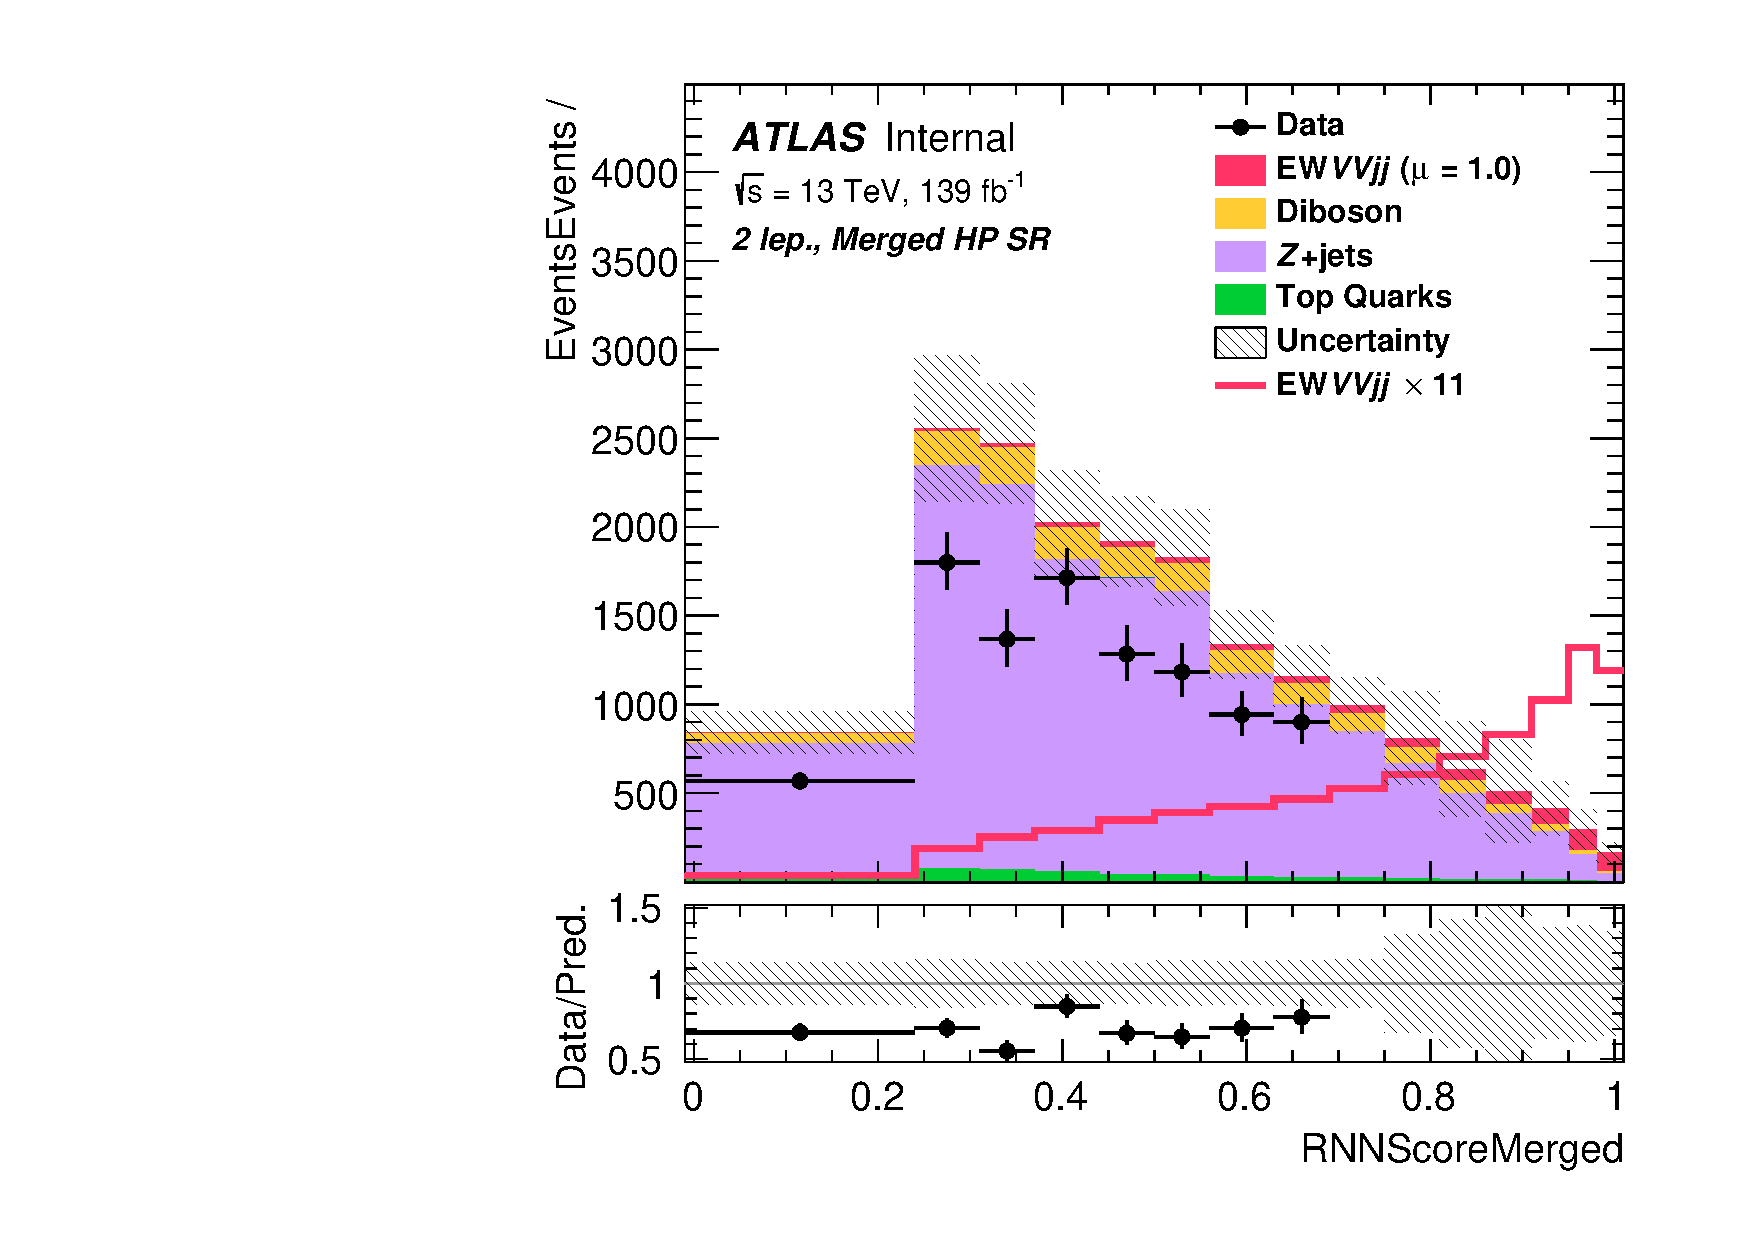
\includegraphics[width=0.35\textwidth]{figures/2lep/FitResults/Region_distRNNScoreMerged_DSRVBSHP_BMin0_J0_incJet1_L2_T0_incFat1_Y6051_incTag1_Fat1_Prefit.pdf}
    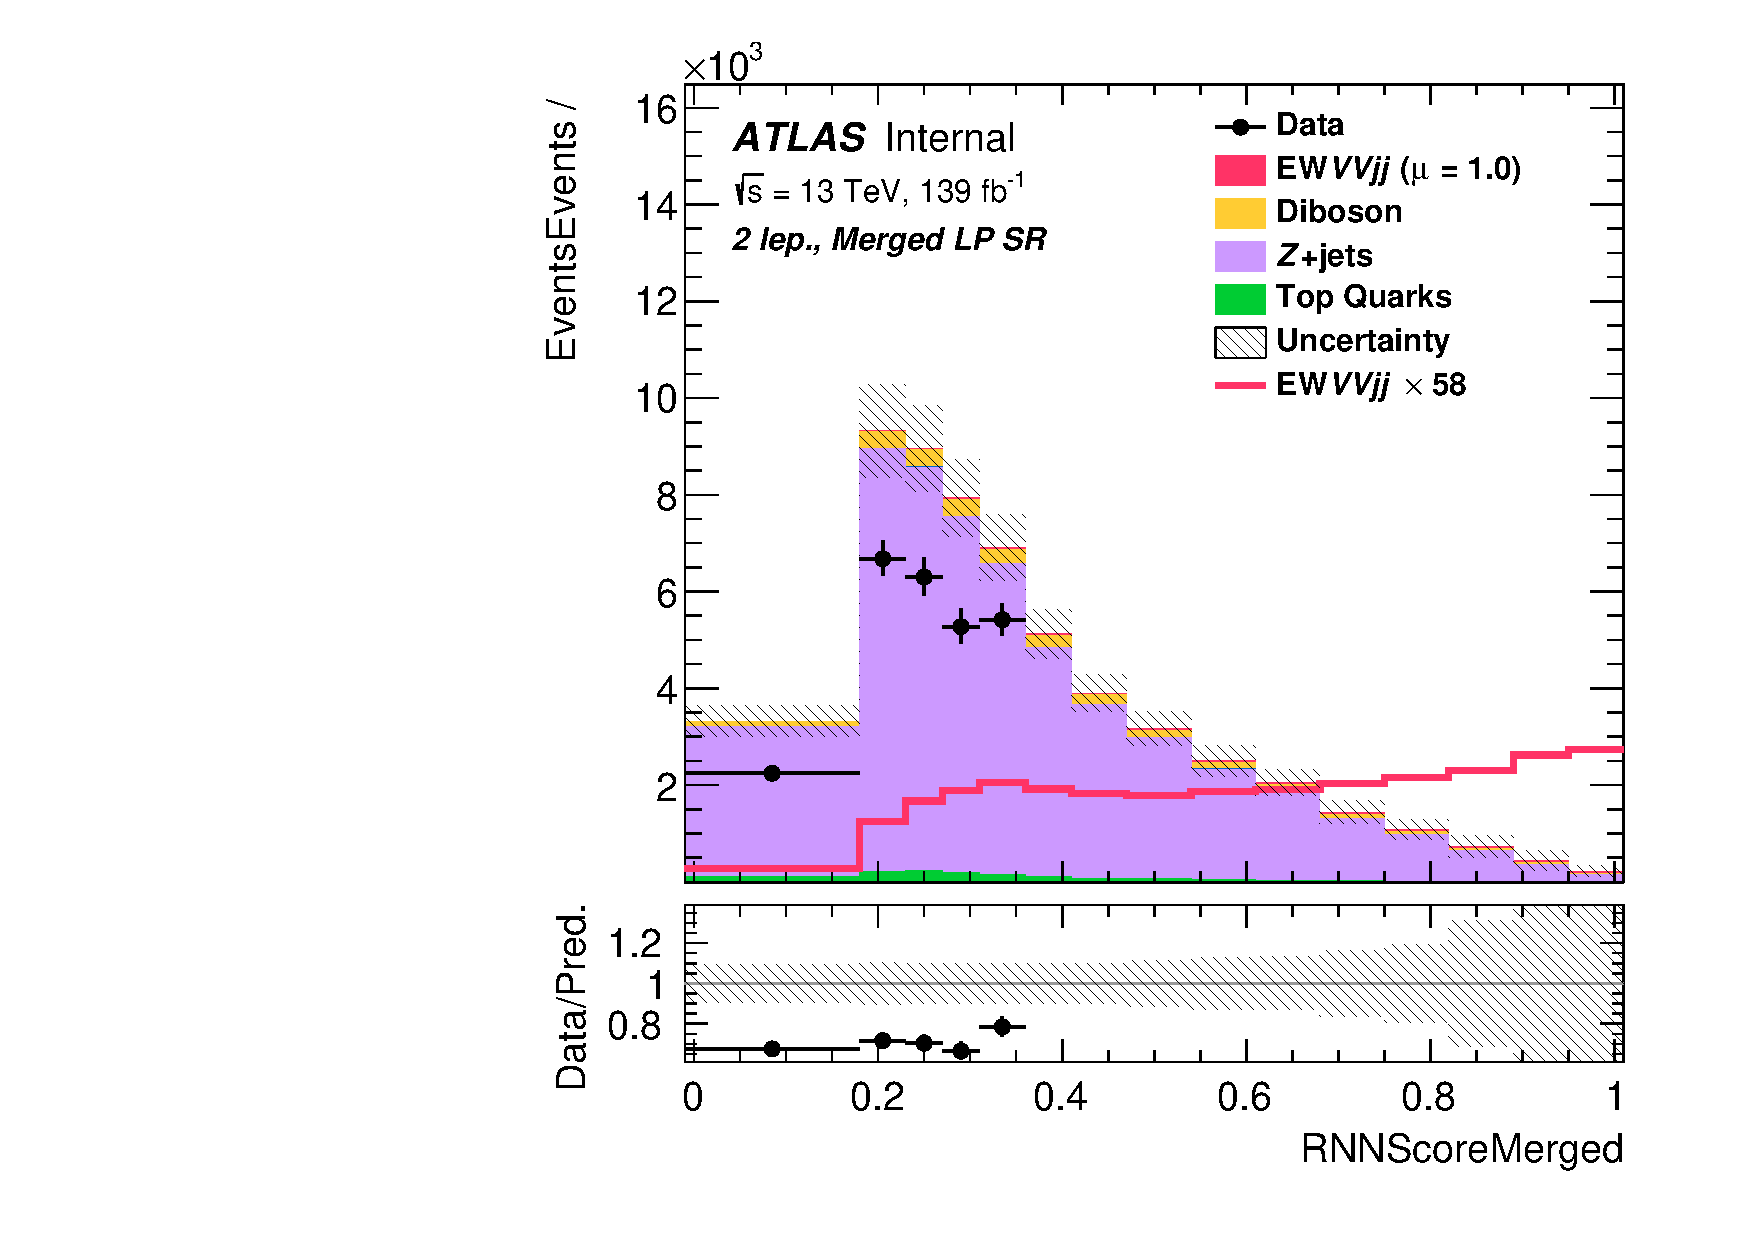
\includegraphics[width=0.35\textwidth]{figures/2lep/FitResults/Region_distRNNScoreMerged_DSRVBSLP_BMin0_J0_incJet1_L2_T0_incFat1_Y6051_incTag1_Fat1_Prefit.pdf}
    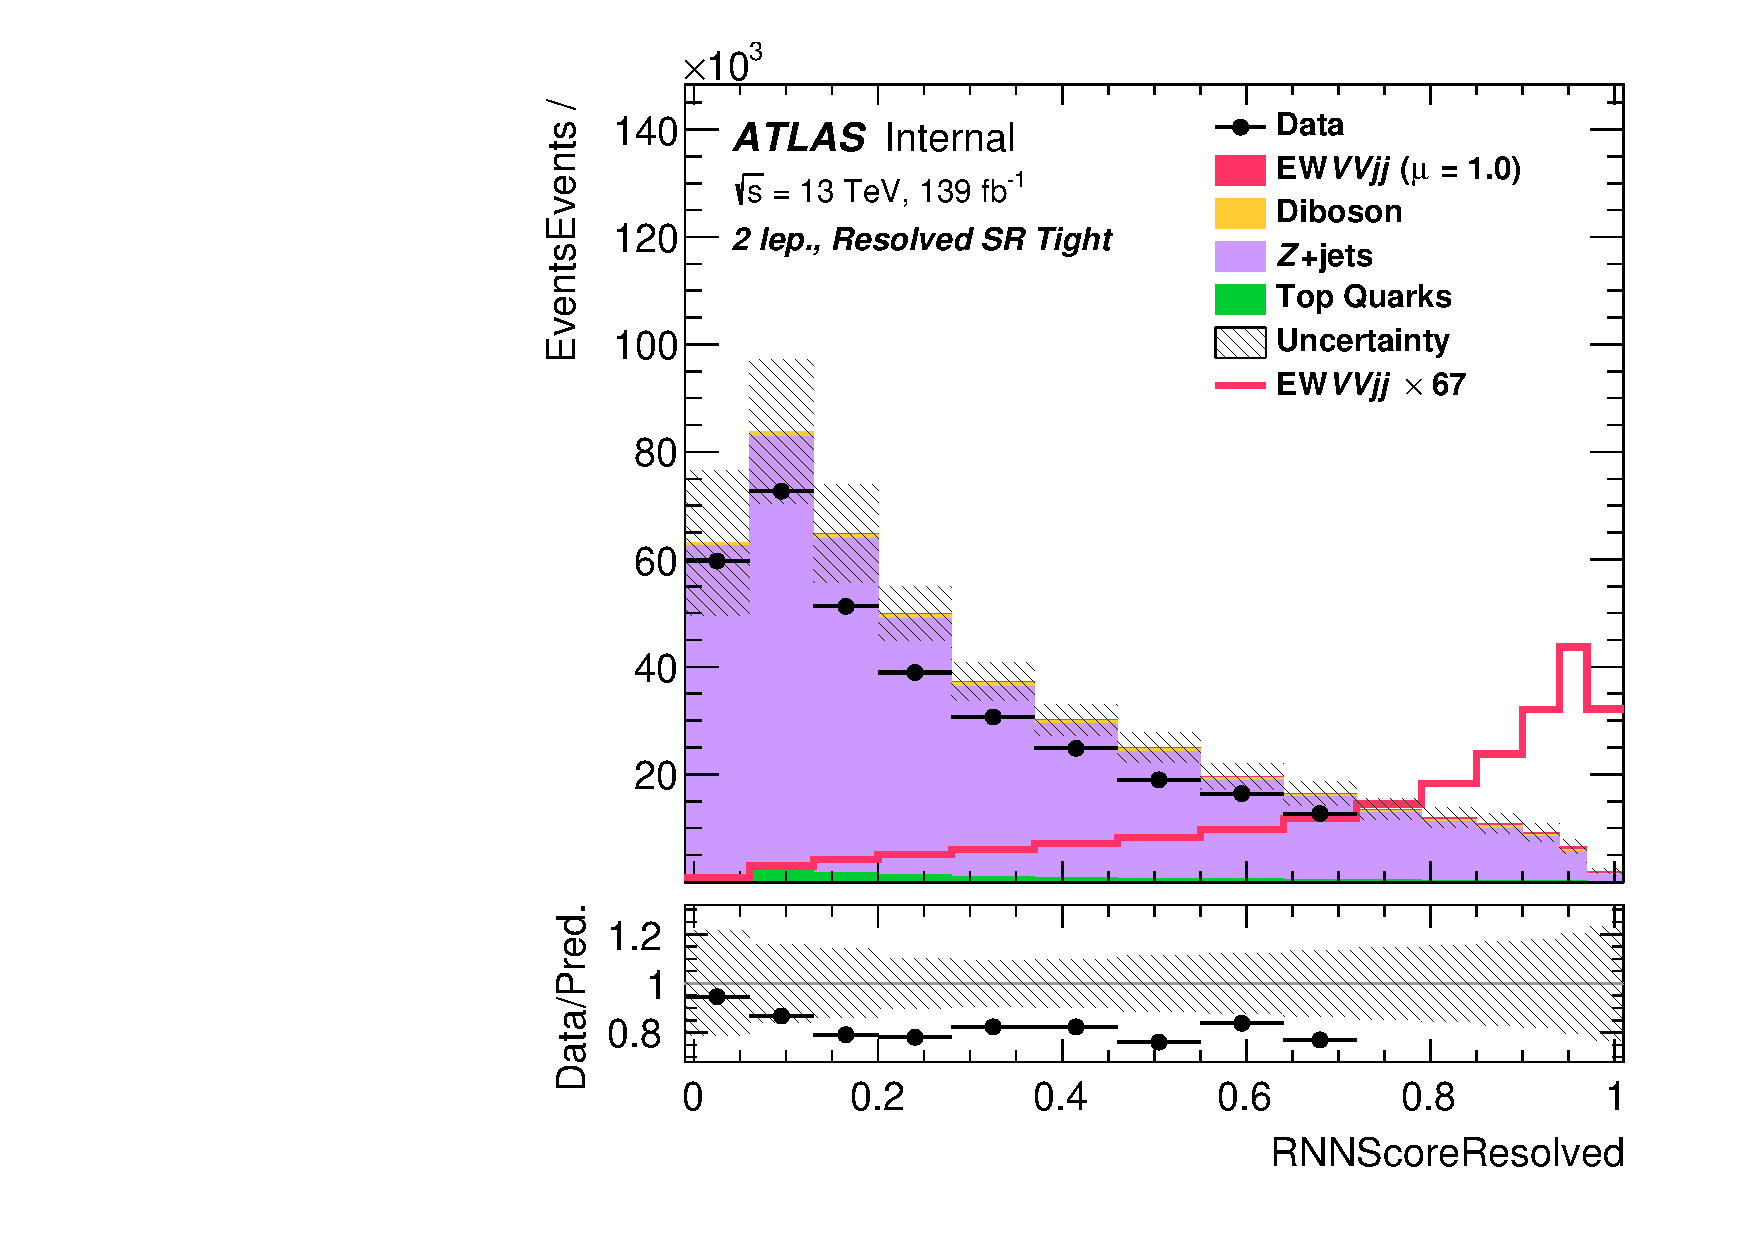
\includegraphics[width=0.35\textwidth]{figures/2lep/FitResults/Region_distRNNScoreResolved_DSRVBSFid_BMin0_T0_Y6051_incTag1_J2_L2_incJet1_Prefit.pdf}
    \\
    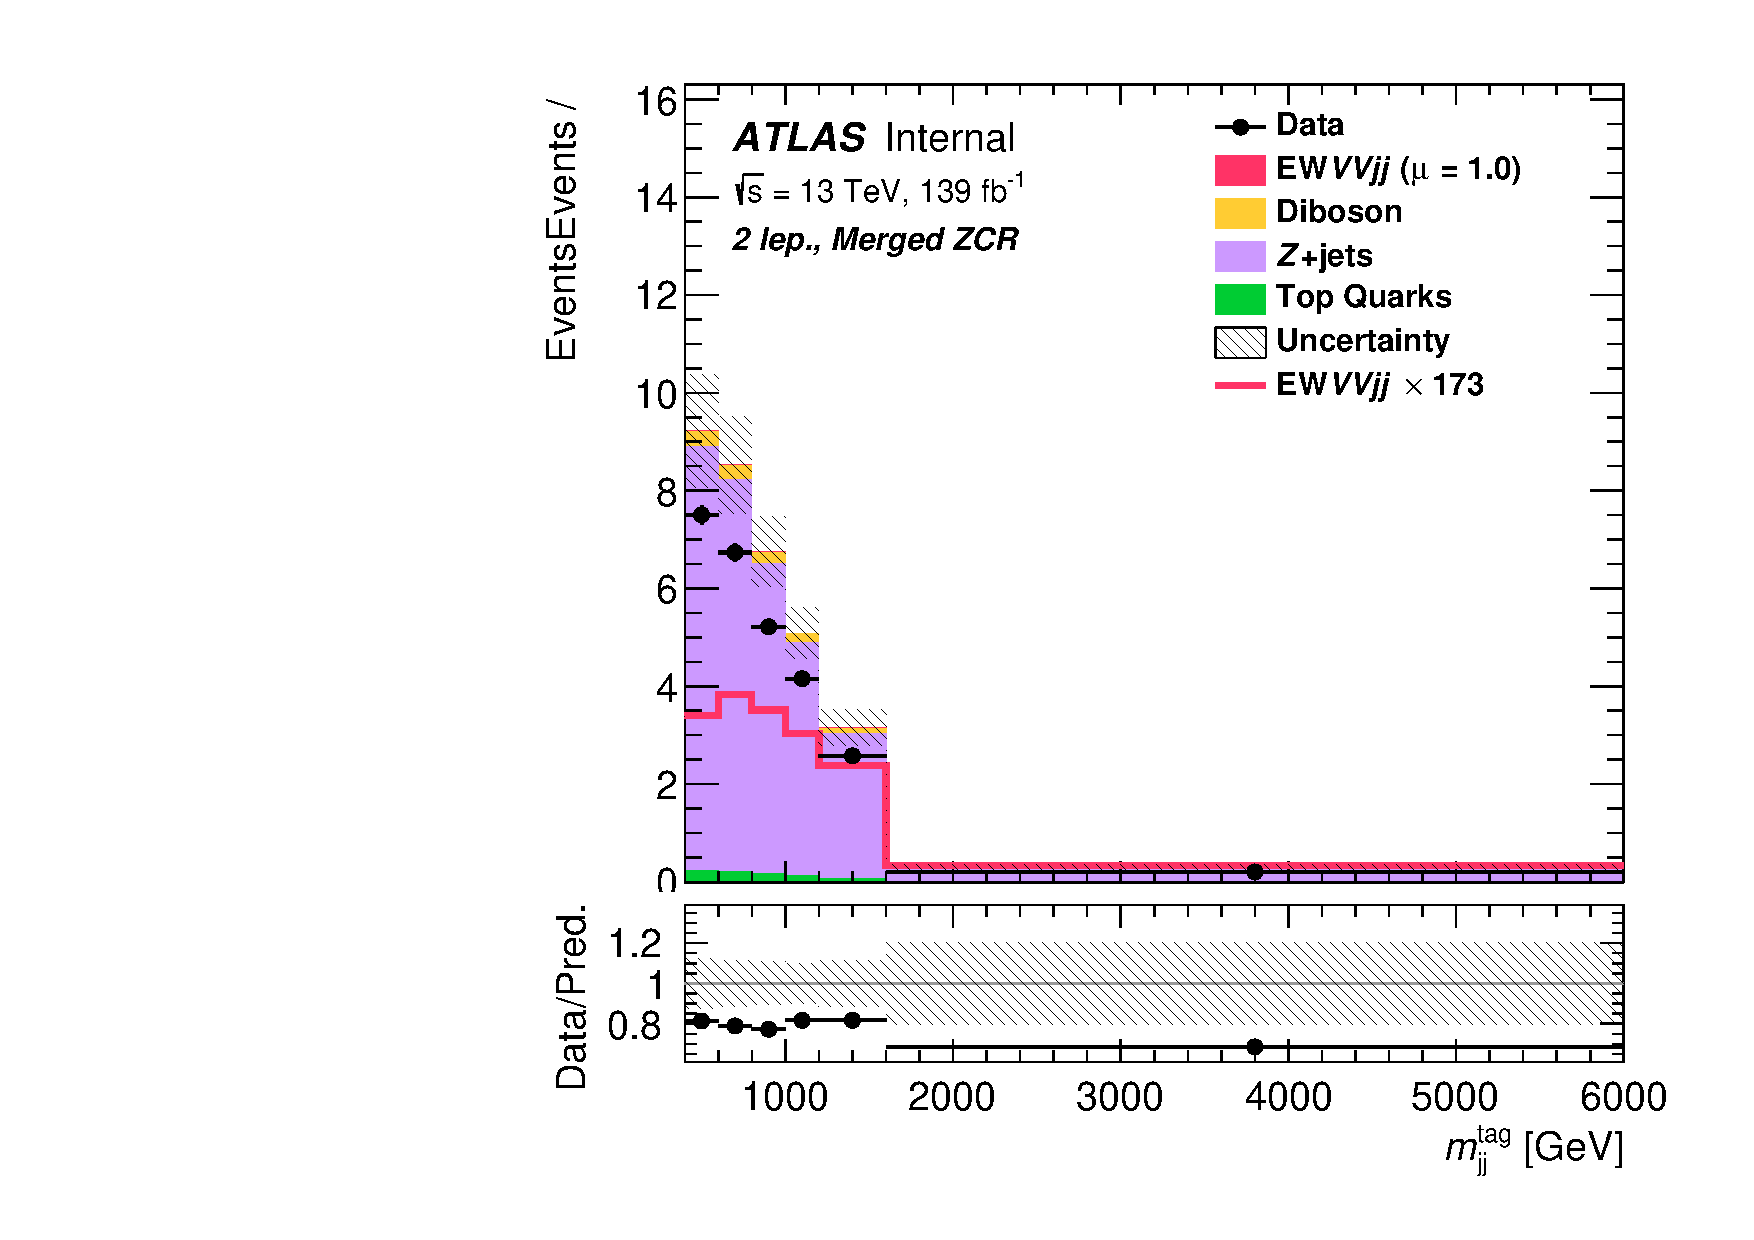
\includegraphics[width=0.35\textwidth]{figures/2lep/FitResults/Region_distMTagMerJets_DCRVjet_BMin0_J0_incJet1_L2_T0_incFat1_Y6051_incTag1_Fat1_Prefit.pdf}
    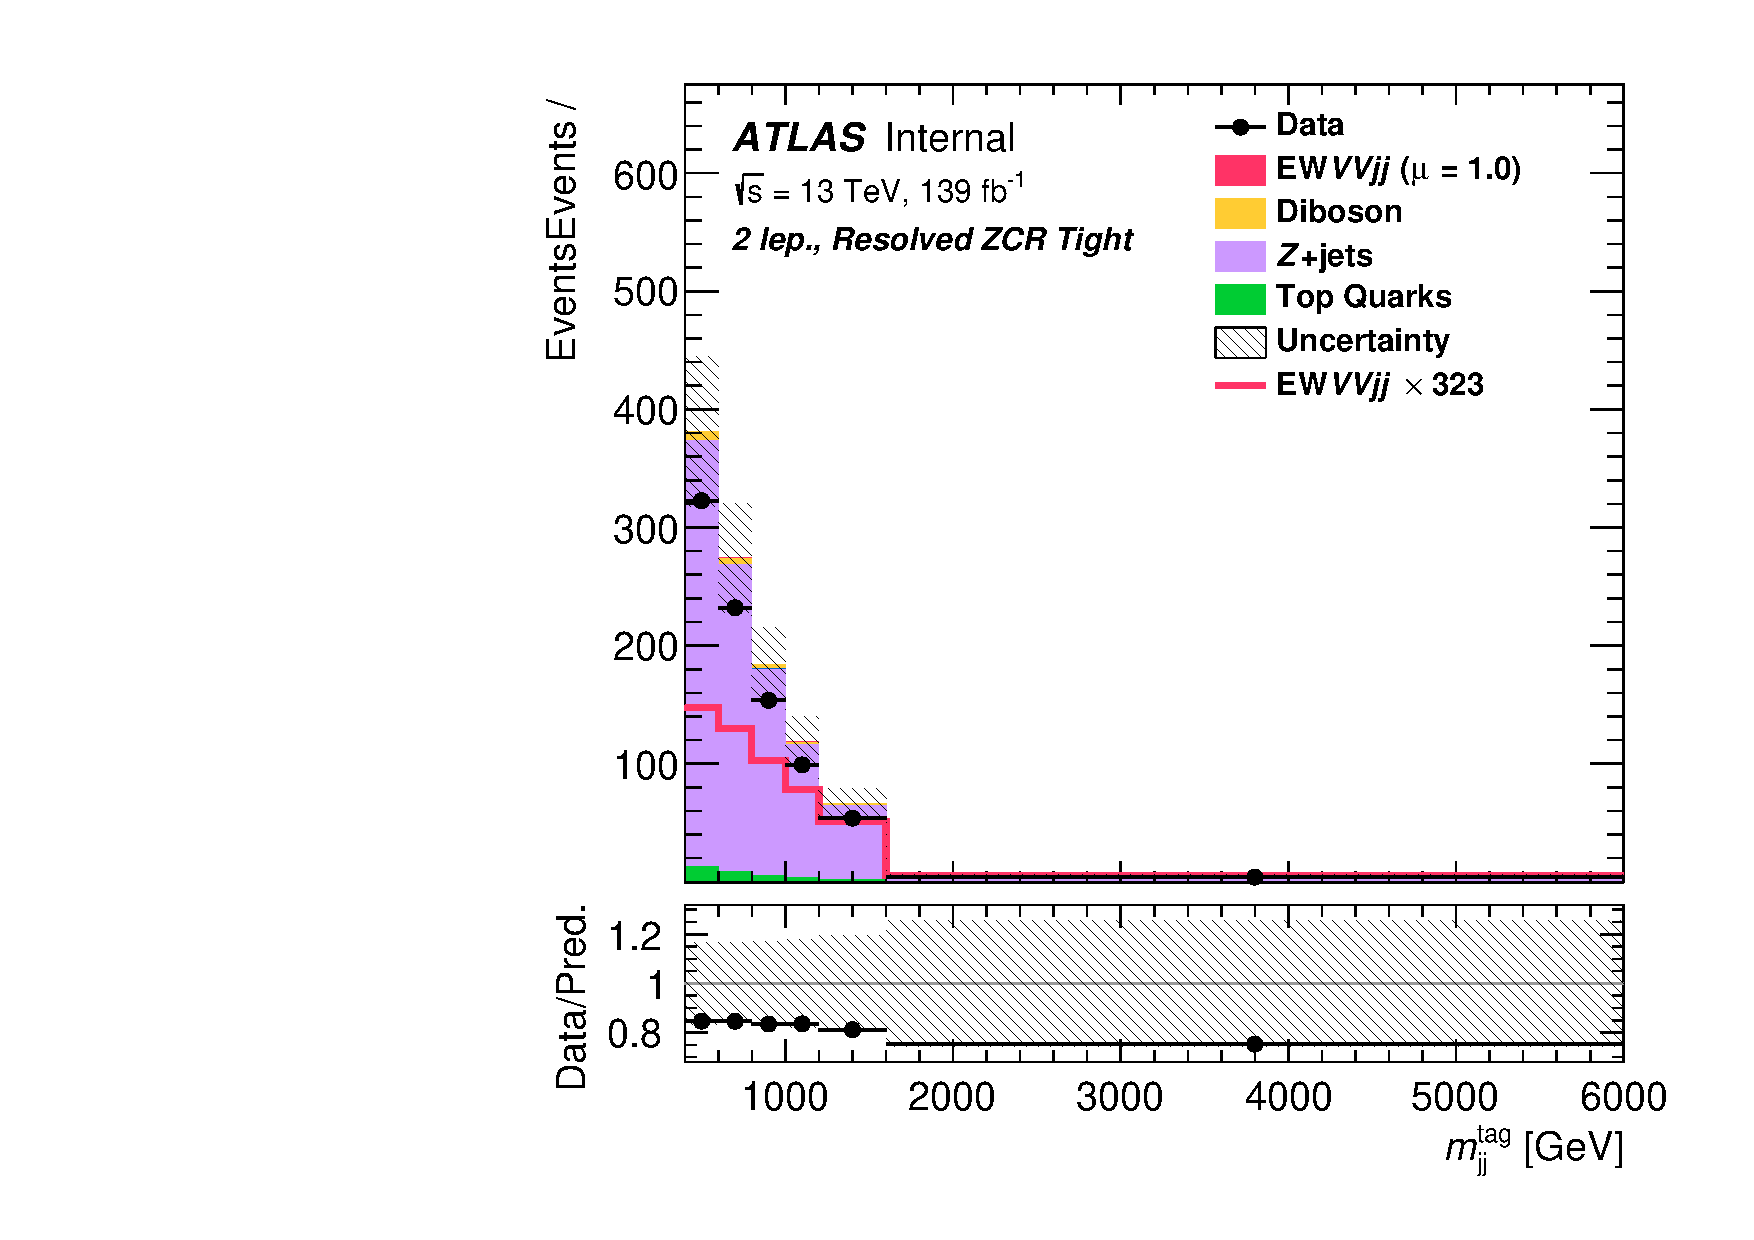
\includegraphics[width=0.35\textwidth]{figures/2lep/FitResults/Region_distMTagResJets_DCRVjetFid_BMin0_T0_Y6051_incTag1_J2_L2_incJet1_Prefit.pdf}
    \caption{Prefit plots for the 2 lepton channel. Data is blinded in the right bins that contain 75\% signal.}
       \label{fig:fit_2lep_prefit}
\end{figure}
\clearpage

\subsection{Postfit plots}
Figure~\ref{fig:fit_2lep_postfit} shows the post-fit plots of the analysis regions entering in the 2-lep fit only model;
The fit is performed with only the left-bins, which are the bins that contain only 75\% signal.

\begin{figure}[ht]
    \centering
    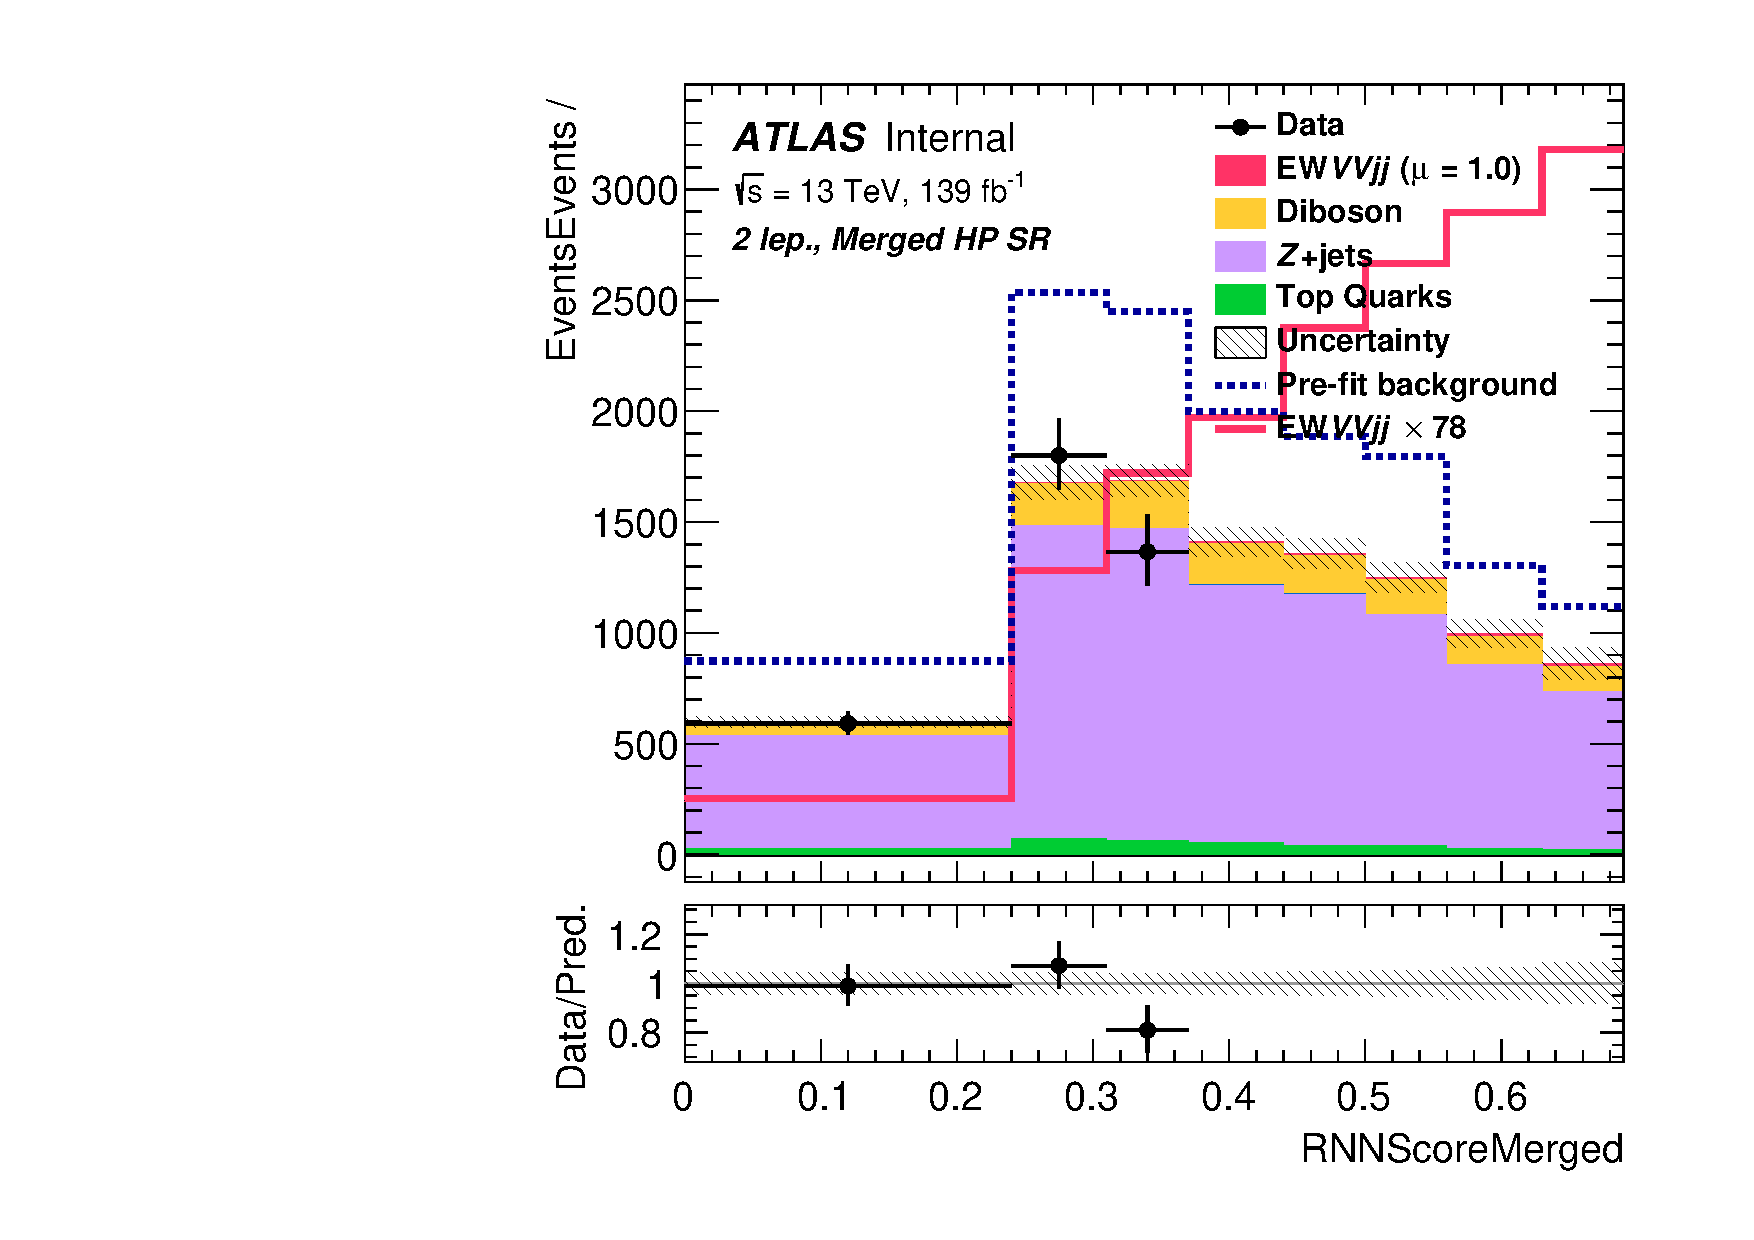
\includegraphics[width=0.35\textwidth]{figures/2lep/FitResults/Region_distRNNScoreMerged_DSRVBSHP_BMin0_J0_incJet1_L2_T0_incFat1_Y6051_incTag1_Fat1_GlobalFit_unconditionnal_mu1.pdf}
    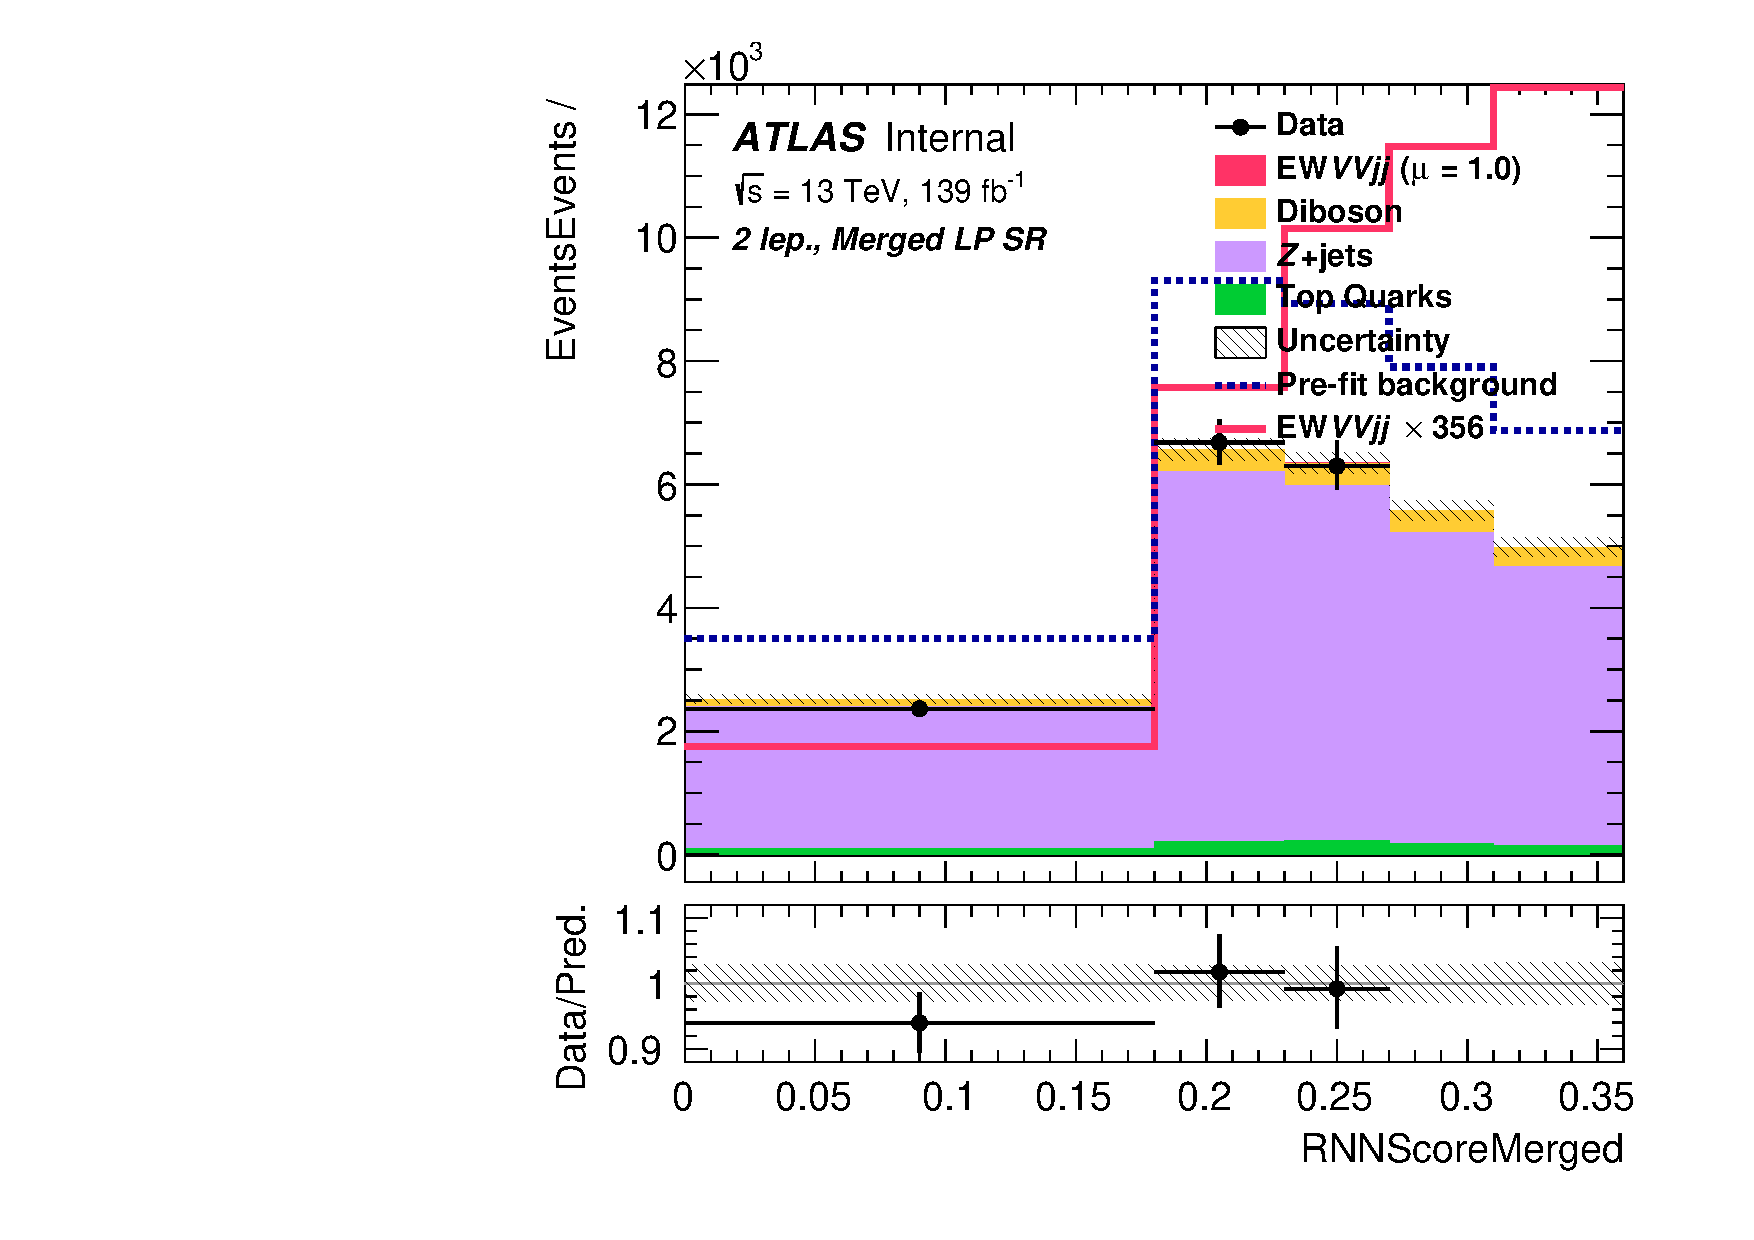
\includegraphics[width=0.35\textwidth]{figures/2lep/FitResults/Region_distRNNScoreMerged_DSRVBSLP_BMin0_J0_incJet1_L2_T0_incFat1_Y6051_incTag1_Fat1_GlobalFit_unconditionnal_mu1.pdf}
    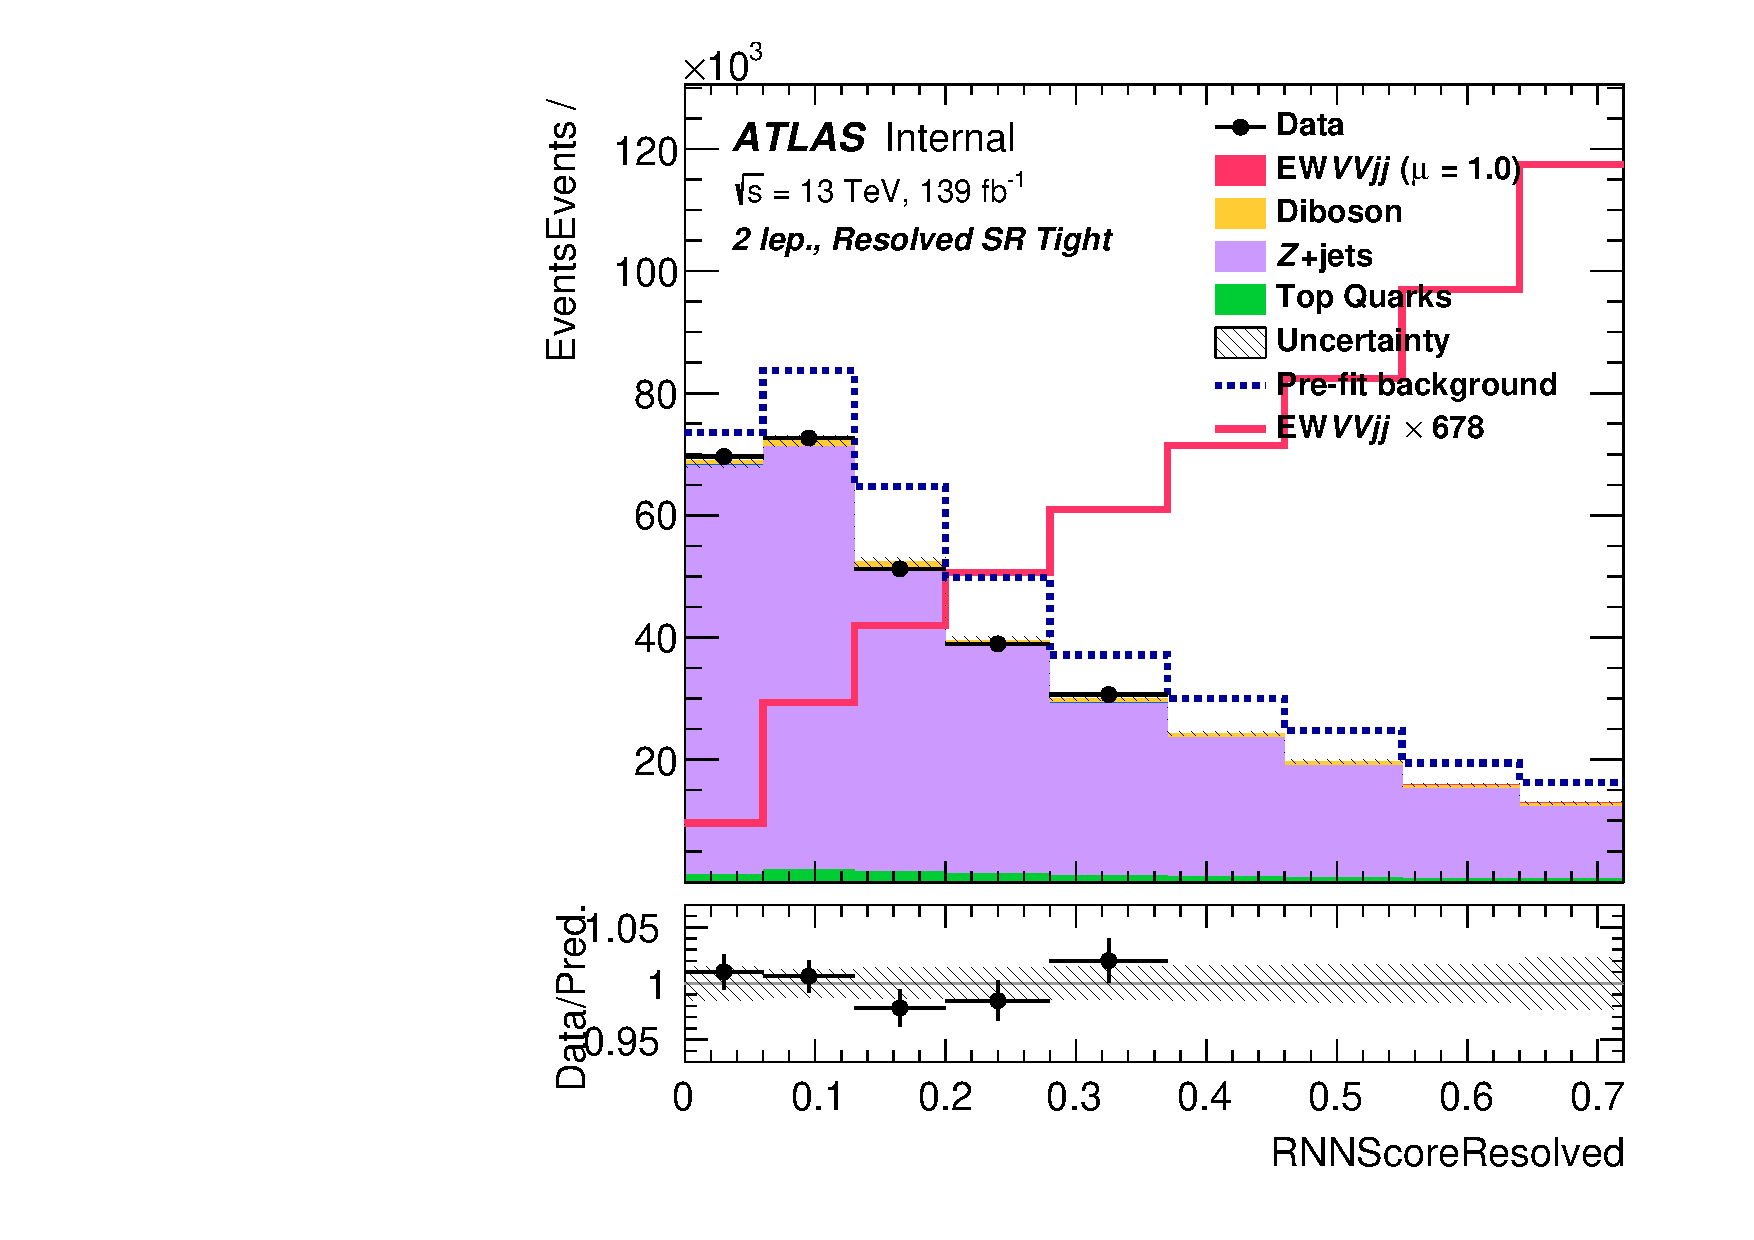
\includegraphics[width=0.35\textwidth]{figures/2lep/FitResults/Region_distRNNScoreResolved_DSRVBSFid_BMin0_T0_Y6051_incTag1_J2_L2_incJet1_GlobalFit_unconditionnal_mu1.pdf}
    \\
    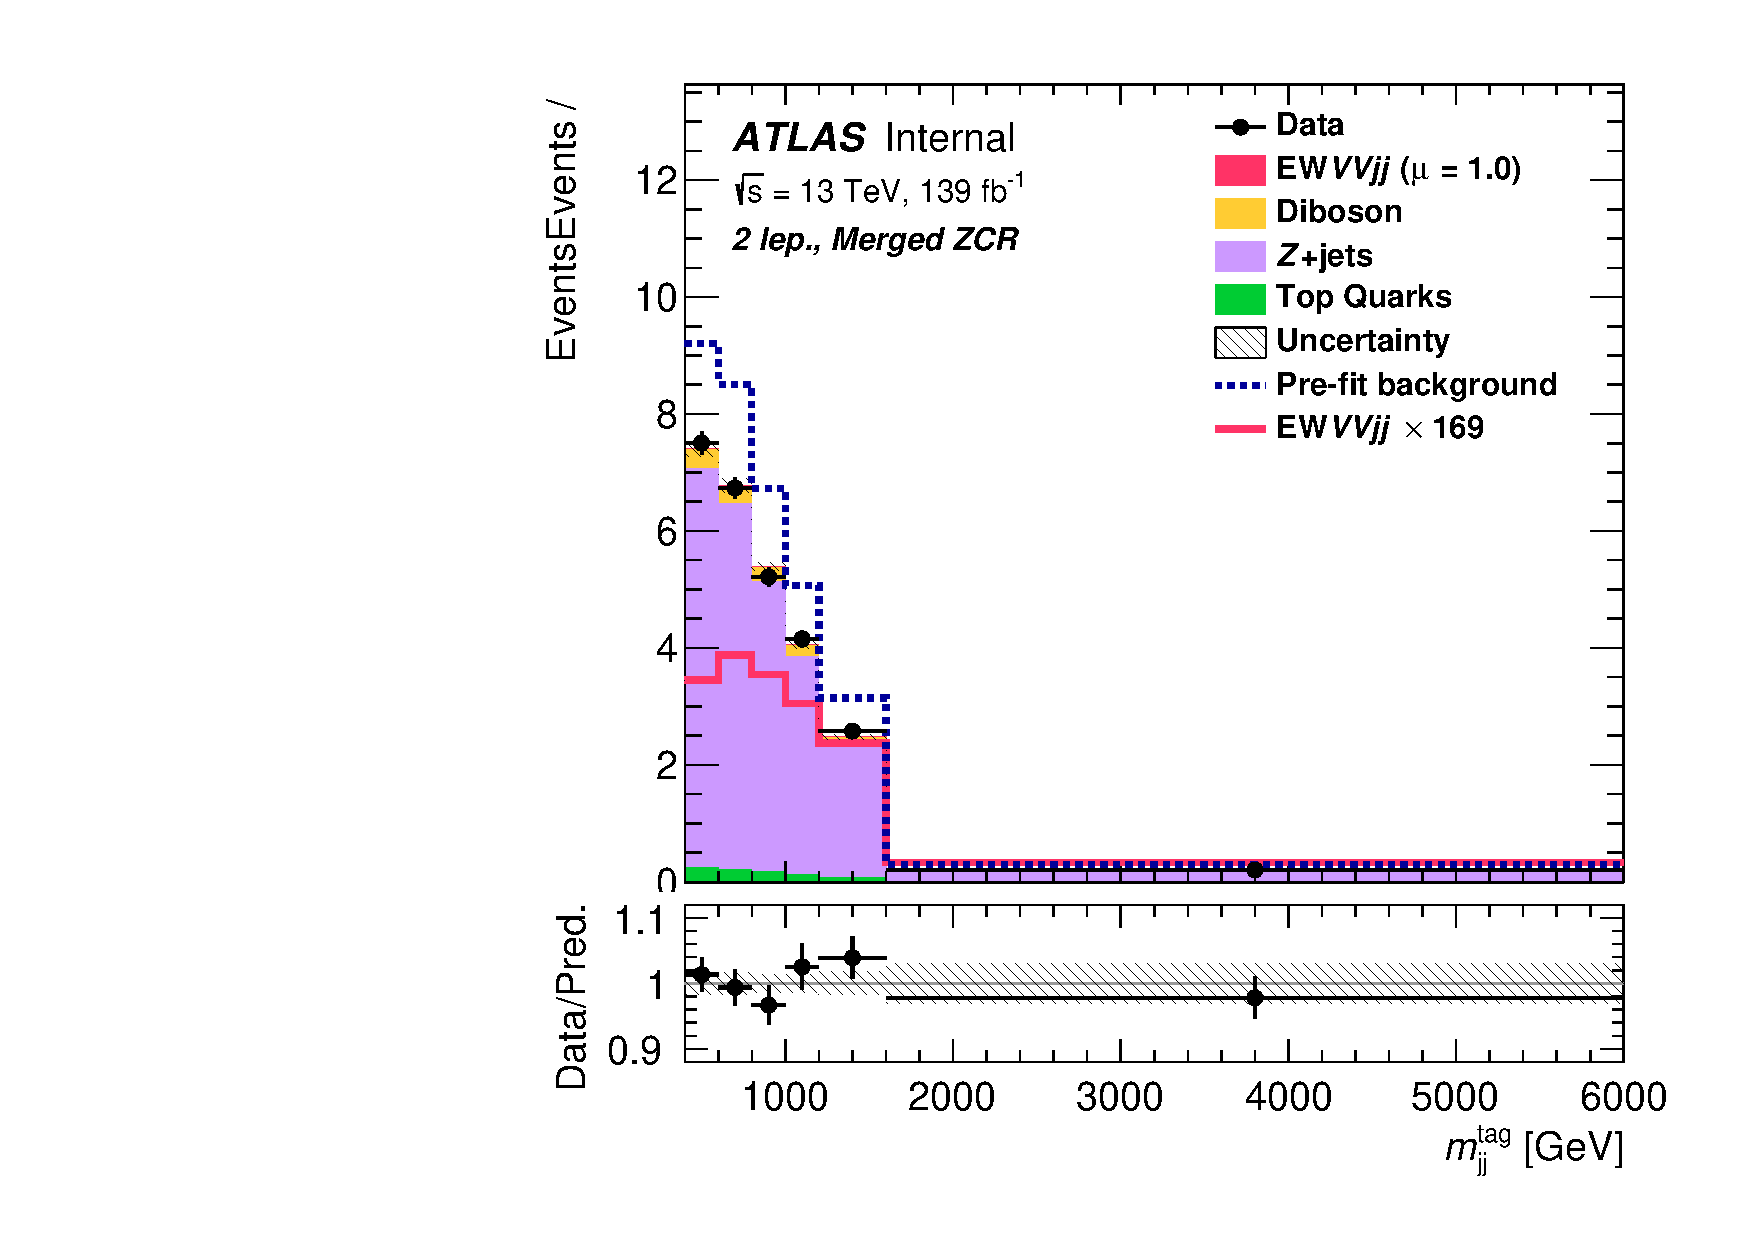
\includegraphics[width=0.35\textwidth]{figures/2lep/FitResults/Region_distMTagMerJets_DCRVjet_BMin0_J0_incJet1_L2_T0_incFat1_Y6051_incTag1_Fat1_GlobalFit_unconditionnal_mu1.pdf}
    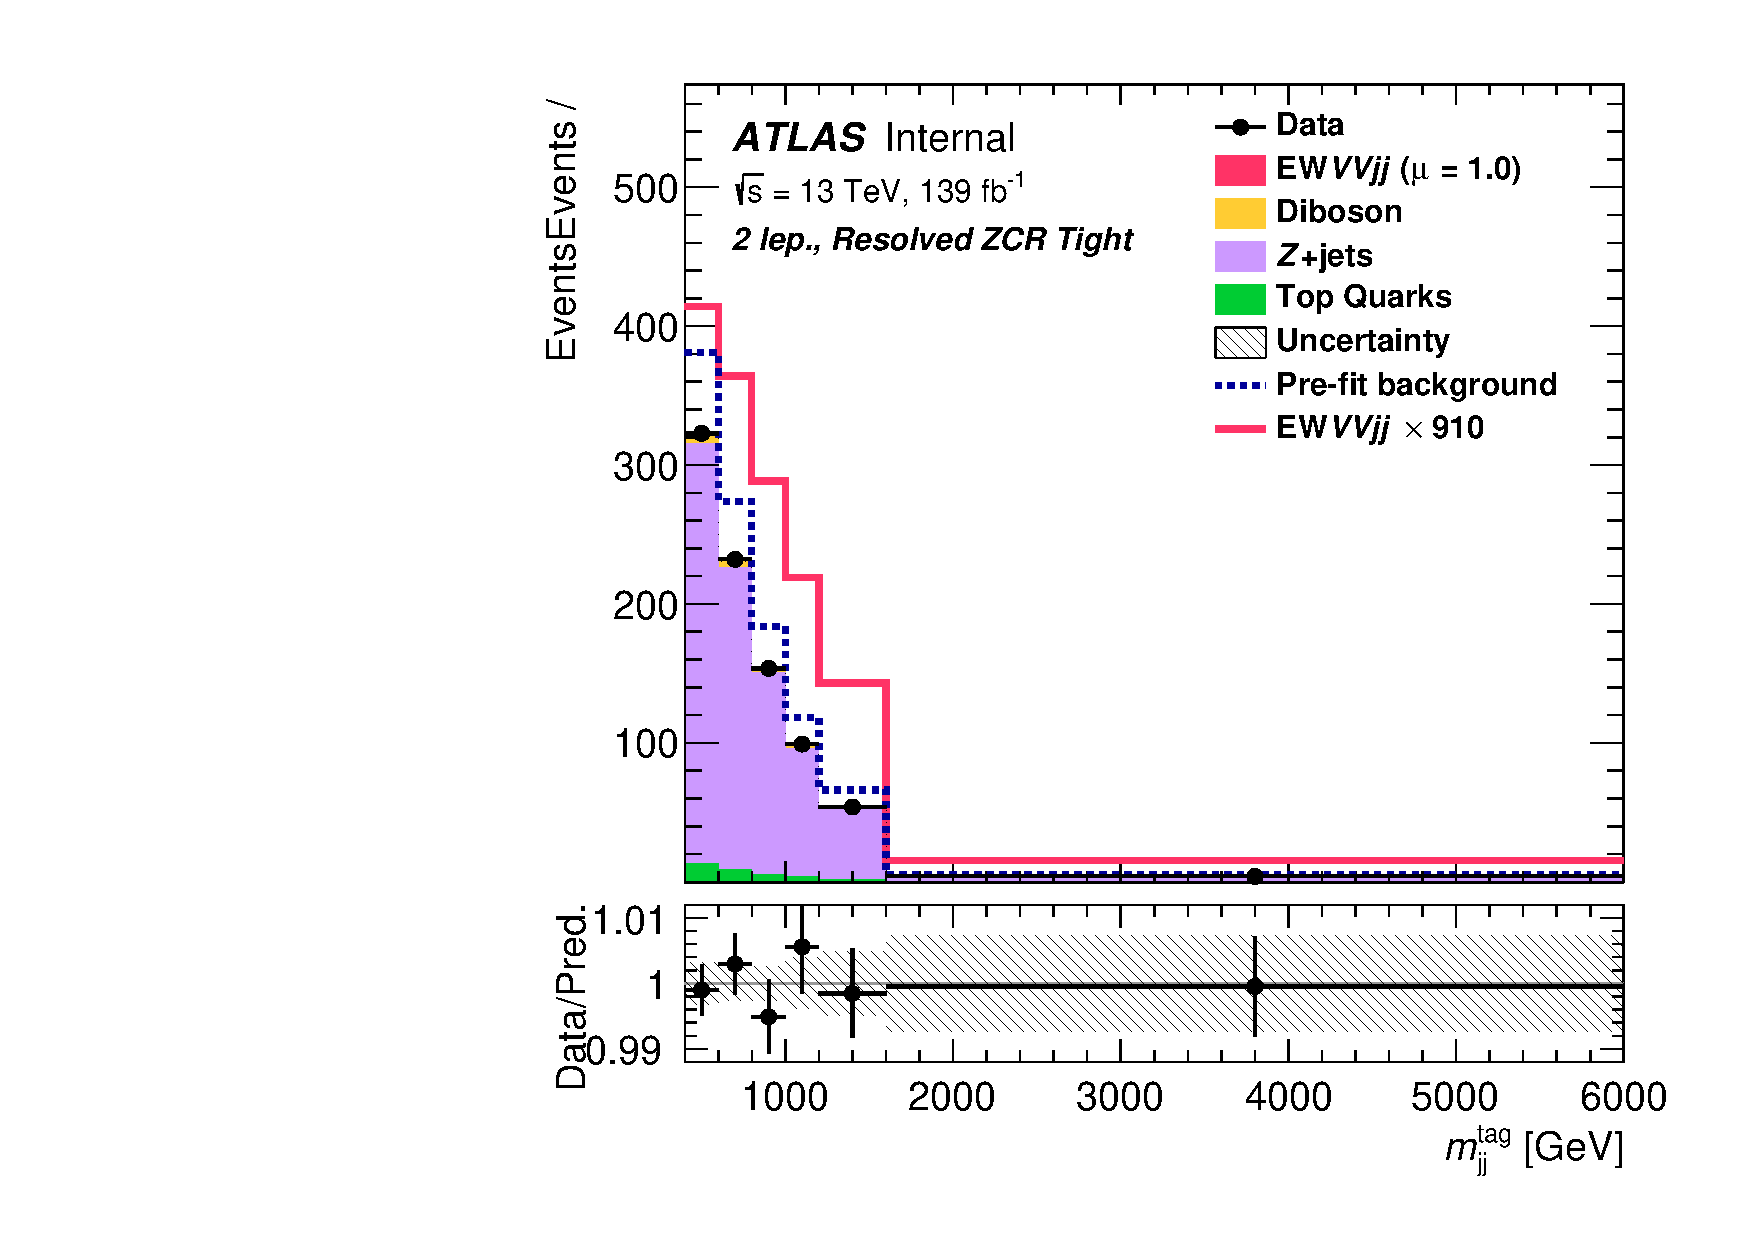
\includegraphics[width=0.35\textwidth]{figures/2lep/FitResults/Region_distMTagResJets_DCRVjetFid_BMin0_T0_Y6051_incTag1_J2_L2_incJet1_GlobalFit_unconditionnal_mu1.pdf}
    \caption{Prefit plots for the 2 lepton channel. Data is blinded in the right bins that contain 75\% signal.}
       \label{fig:fit_2lep_prefit}
\end{figure}
\clearpage

\subsection{Asimov Fit Results}
A fit to the full range of SRs using Asimov data is performed only with the 2 lepton channel.

Figures \ref{fig:fit_2lep_fcc_asimov}-\ref{fig:fit_2lep_corr_all}-\ref{fig:fit_2lep_ranking_all}
show the pulls, the correlation and the ranking respectively of the NPs used in the fit.

In particular, the following constraints have been found:
\begin{itemize}
       \item \texttt{SysTheoryQCD\_Z} is the QCD scale uncertainty on the Z+jets samples.
       The large shape impact of the resolved SR cause this constraint;
       we will provide more checks in section \ref{sec:fit_decorrStudies}.

       \item \texttt{SysMJJREWEIGHT\_100per} (L2\_Fat1 for merged and L2\_J2 for resolved)
       are the \mjjtag reweighting uncertainties for merged and resolved regions.
       These are large uncertainties and are expected since we take the \mjjtag reweighting as 100\% uncertainties.
       We rely on the constraints coming from data to this uncertainty.

       \item \texttt{SysMODEL\_Z\_MGPy8}
       is the shape difference between Sherpa Z+jets samples (after the \mjjtag reweighting applied)
       and the MadGraph Z+jets samples (no \mjjtag reweighting applied).
       These are expected since there is a well-known modelling difference between two generators.

\end{itemize}

\begin{figure}[ht]
      \centering
        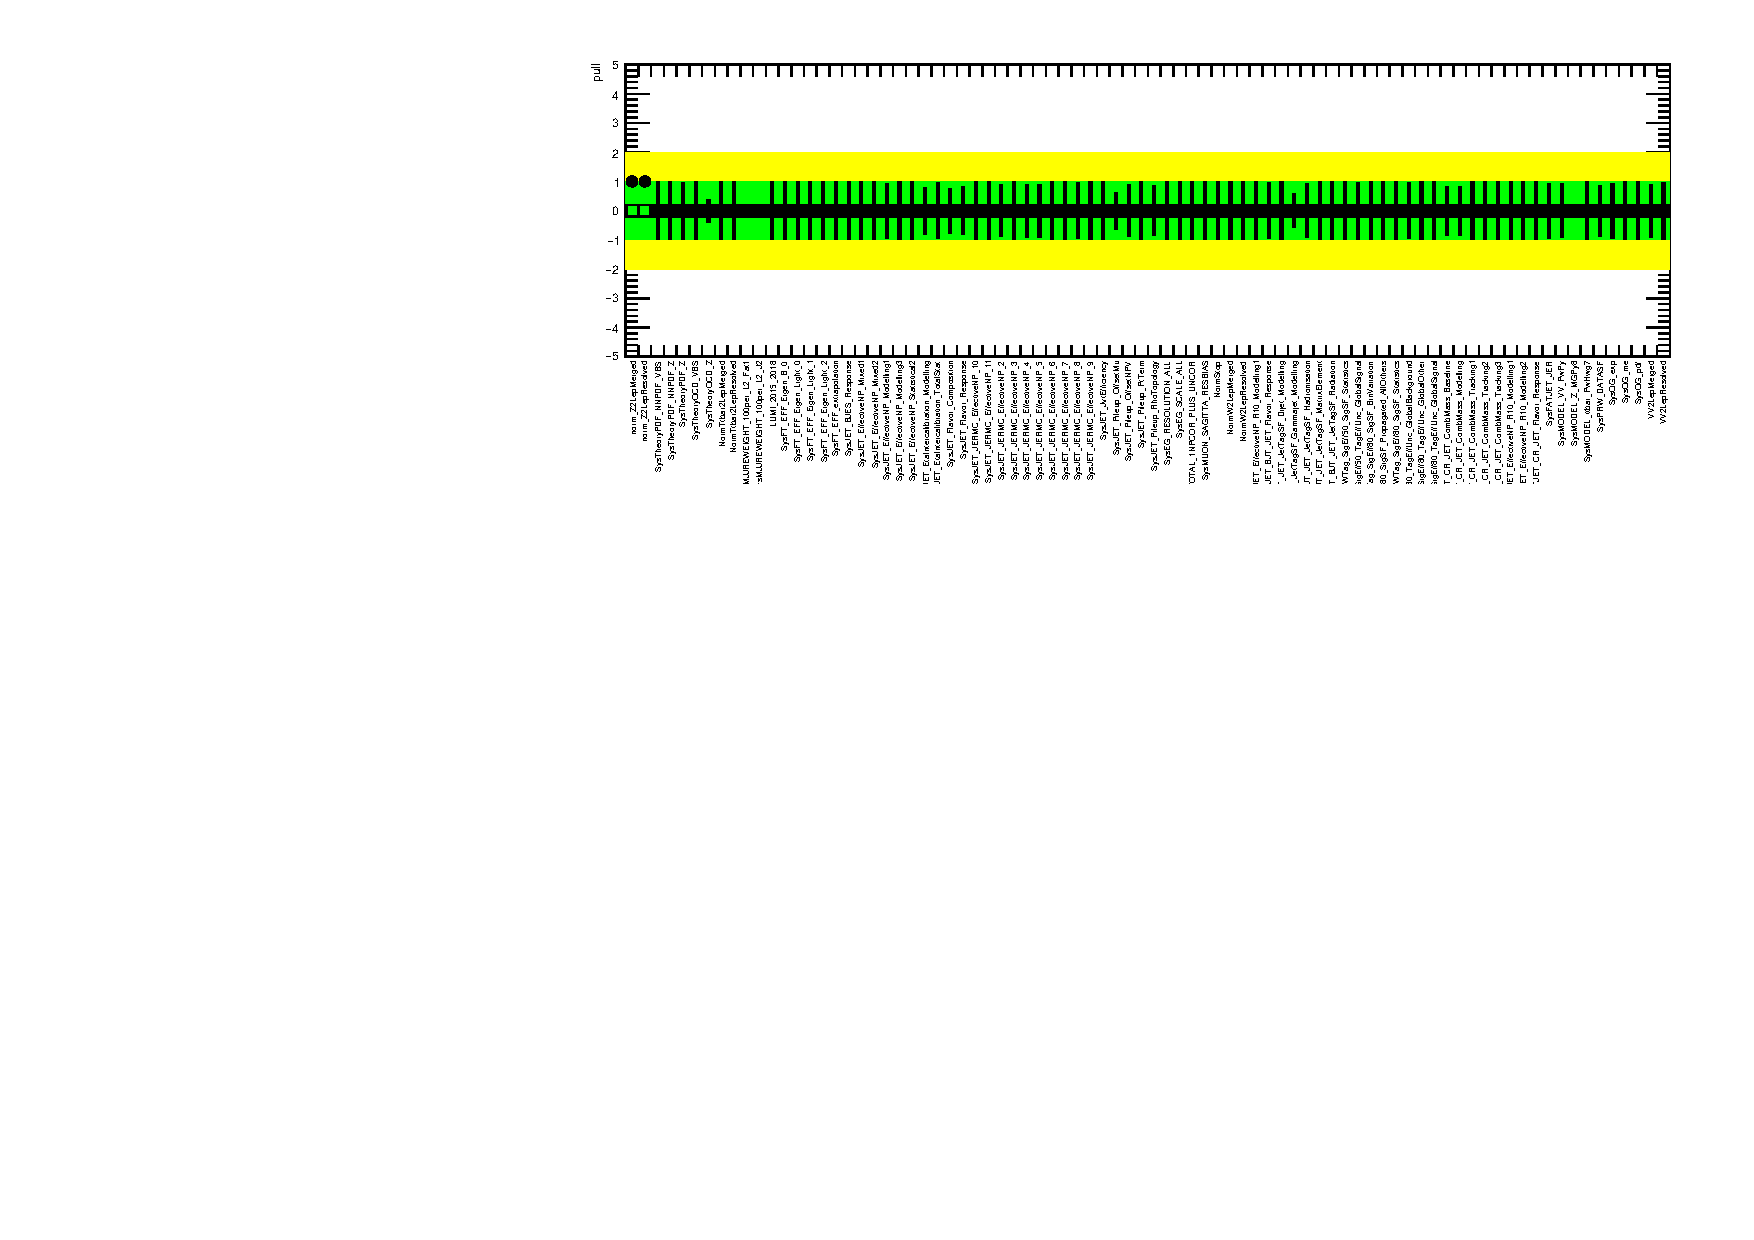
\includegraphics[width=\linewidth]{figures/2lep/FitResults/NP_allExceptGammas_AsimovAllbins.pdf}
        \caption{Fit cross-check, unconditional fit ($\mu=1$) to asimov data for the 2 lepton channel only.}
       \label{fig:fit_2lep_fcc_asimov}
\end{figure}

\begin{figure}[ht]
      \centering
        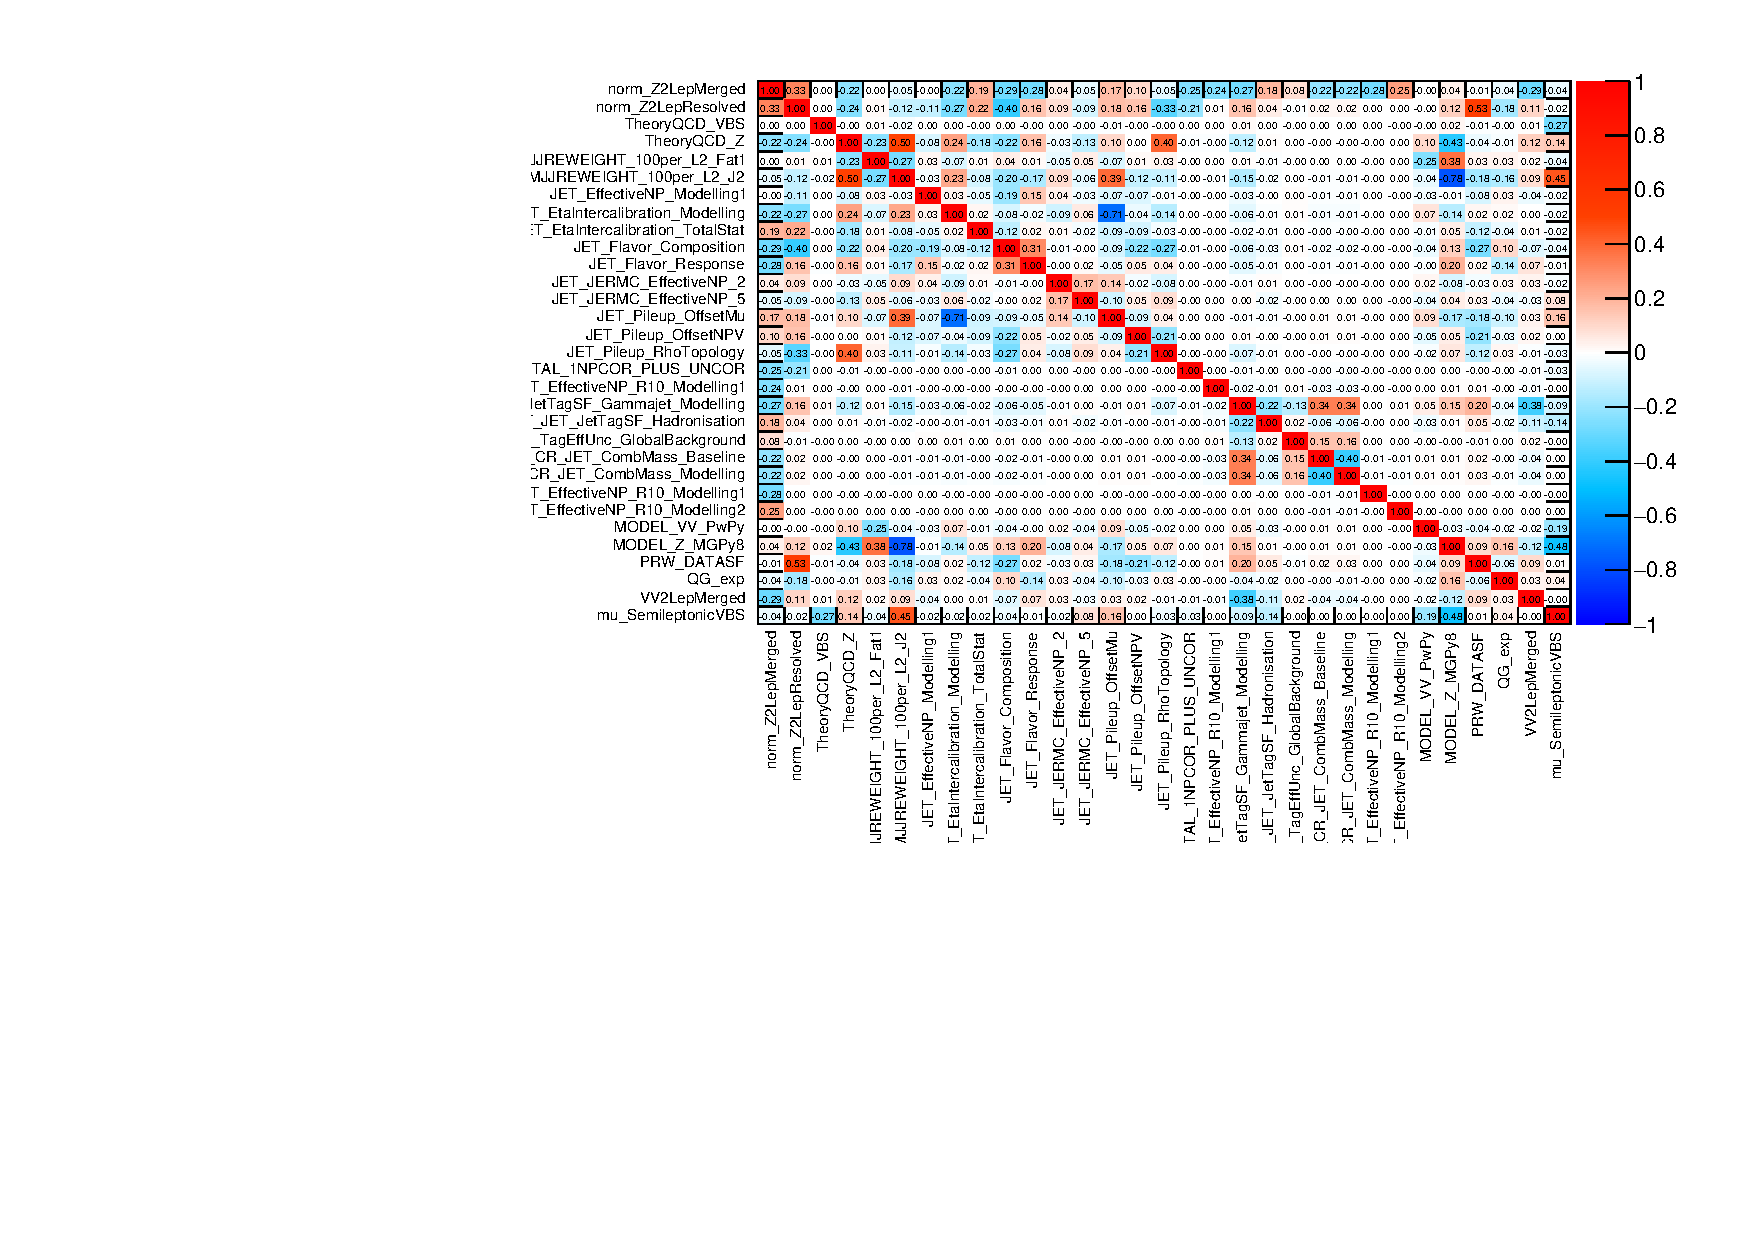
\includegraphics[width=\linewidth]{figures/2lep/FitResults/corr_HighCorrNoMCStat_AsimovAllbins.pdf}
        \caption{Correlations for unconditional fit ($\mu=1$) to asimov data in the full range, for the 2 lepton channel only.}
       \label{fig:fit_2lep_corr_all}
\end{figure}

\begin{figure}[ht]
      \centering
        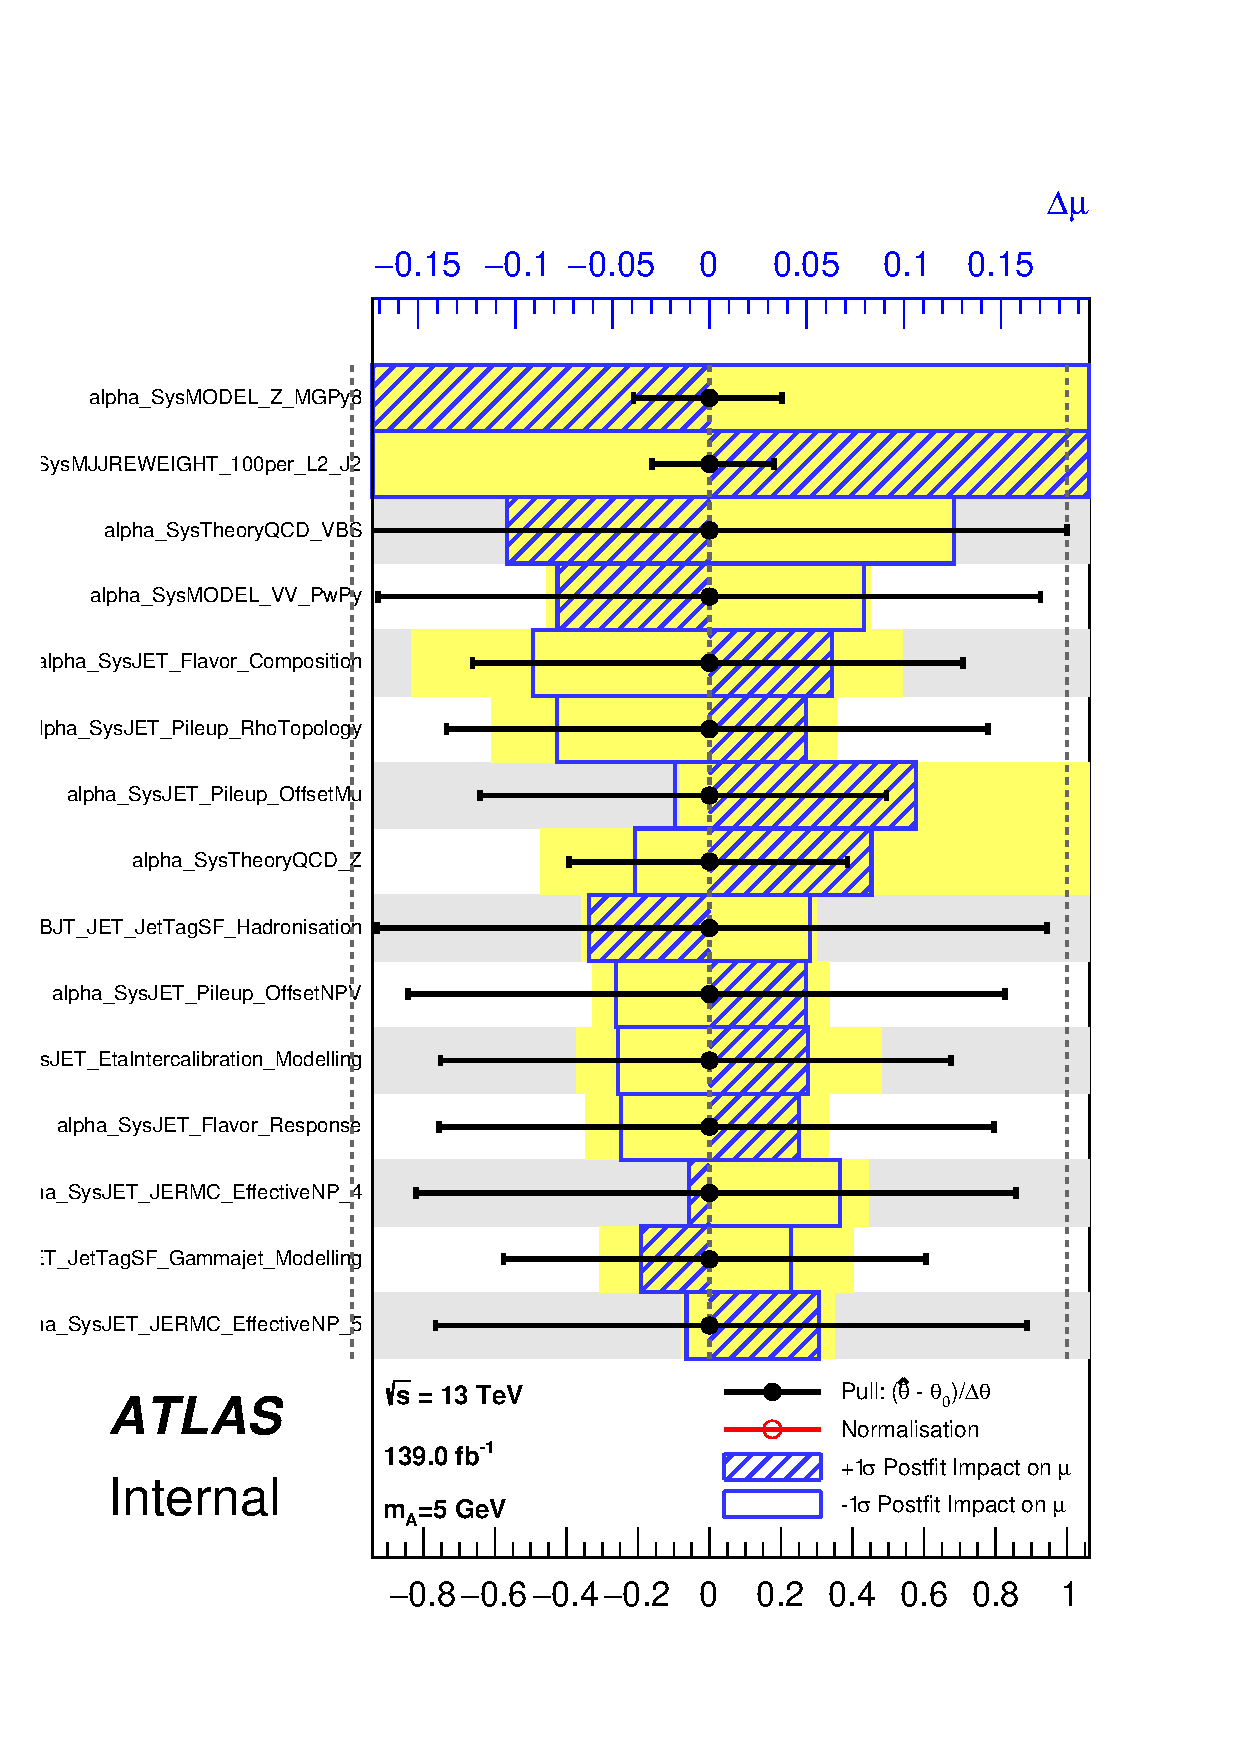
\includegraphics[width=0.5\textwidth]{figures/2lep/FitResults/pulls_mu_SemileptonicVBS_5_AsimovAllbins.pdf}
        \caption{Ranking plot for unconditional fit ($\mu=1$) to asimov data in the full range, for the 2 lepton channel only.}
       \label{fig:fit_2lep_ranking_all}
\end{figure}

\subsection{Left Bins Data Fit Results}

According to the unblinding strategy, the fit model is inspected in the left side of our SRs using data fit;
the goal is to spot some problematic pulls that might appear in the final data fit.

Figures \ref{fig:fit_2lep_fcc_left}-\ref{fig:fit_2lep_corr_left}
show the pulls and the correlations respectively of the NPs used in the fit.

\begin{figure}[ht]
      \centering
        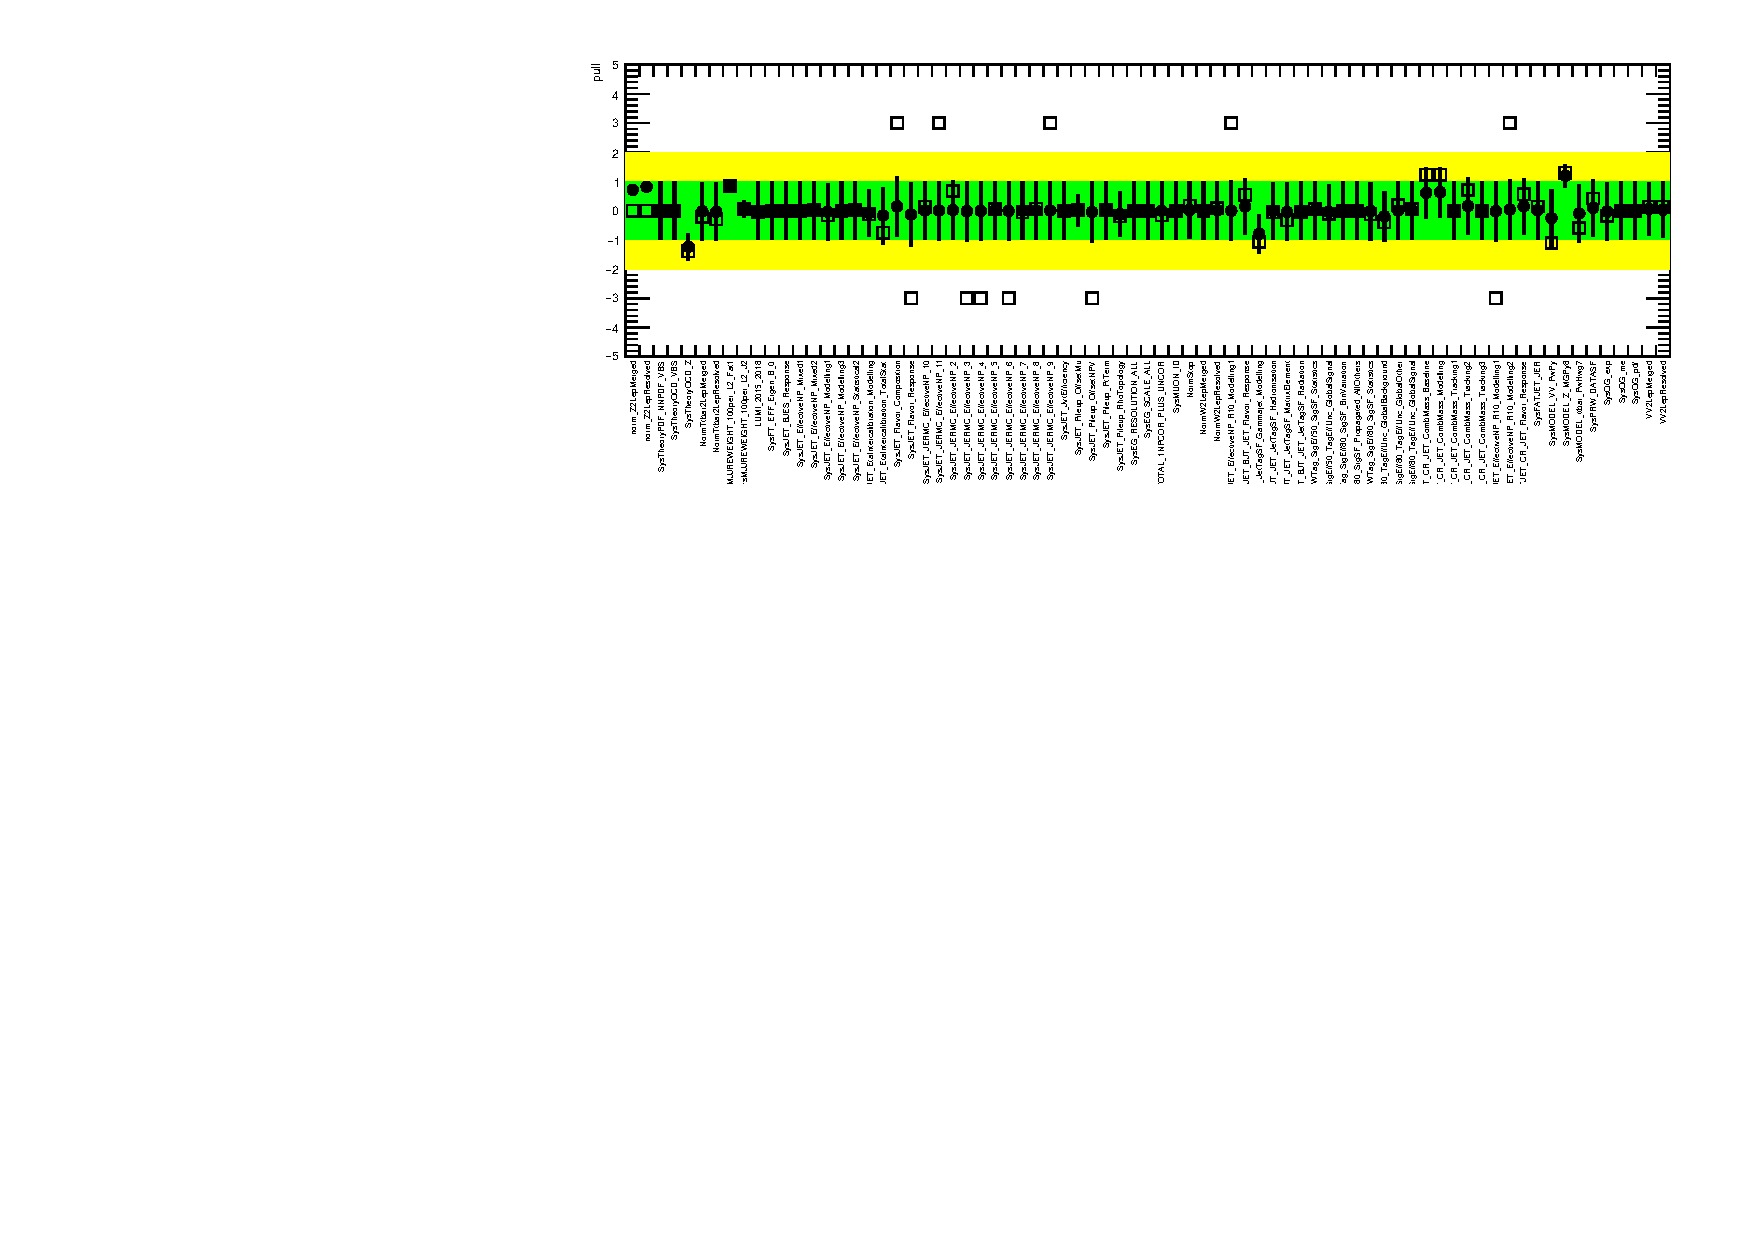
\includegraphics[width=\linewidth]{figures/2lep/FitResults/NP_allExceptGammas_DataLeftBins.pdf}
        \caption{Fit cross-check, unconditional fit ($\mu=1$) to data in the left bins only, for the 2 lepton channel only.}
       \label{fig:fit_2lep_fcc_left}
\end{figure}

\begin{figure}[ht]
      \centering
        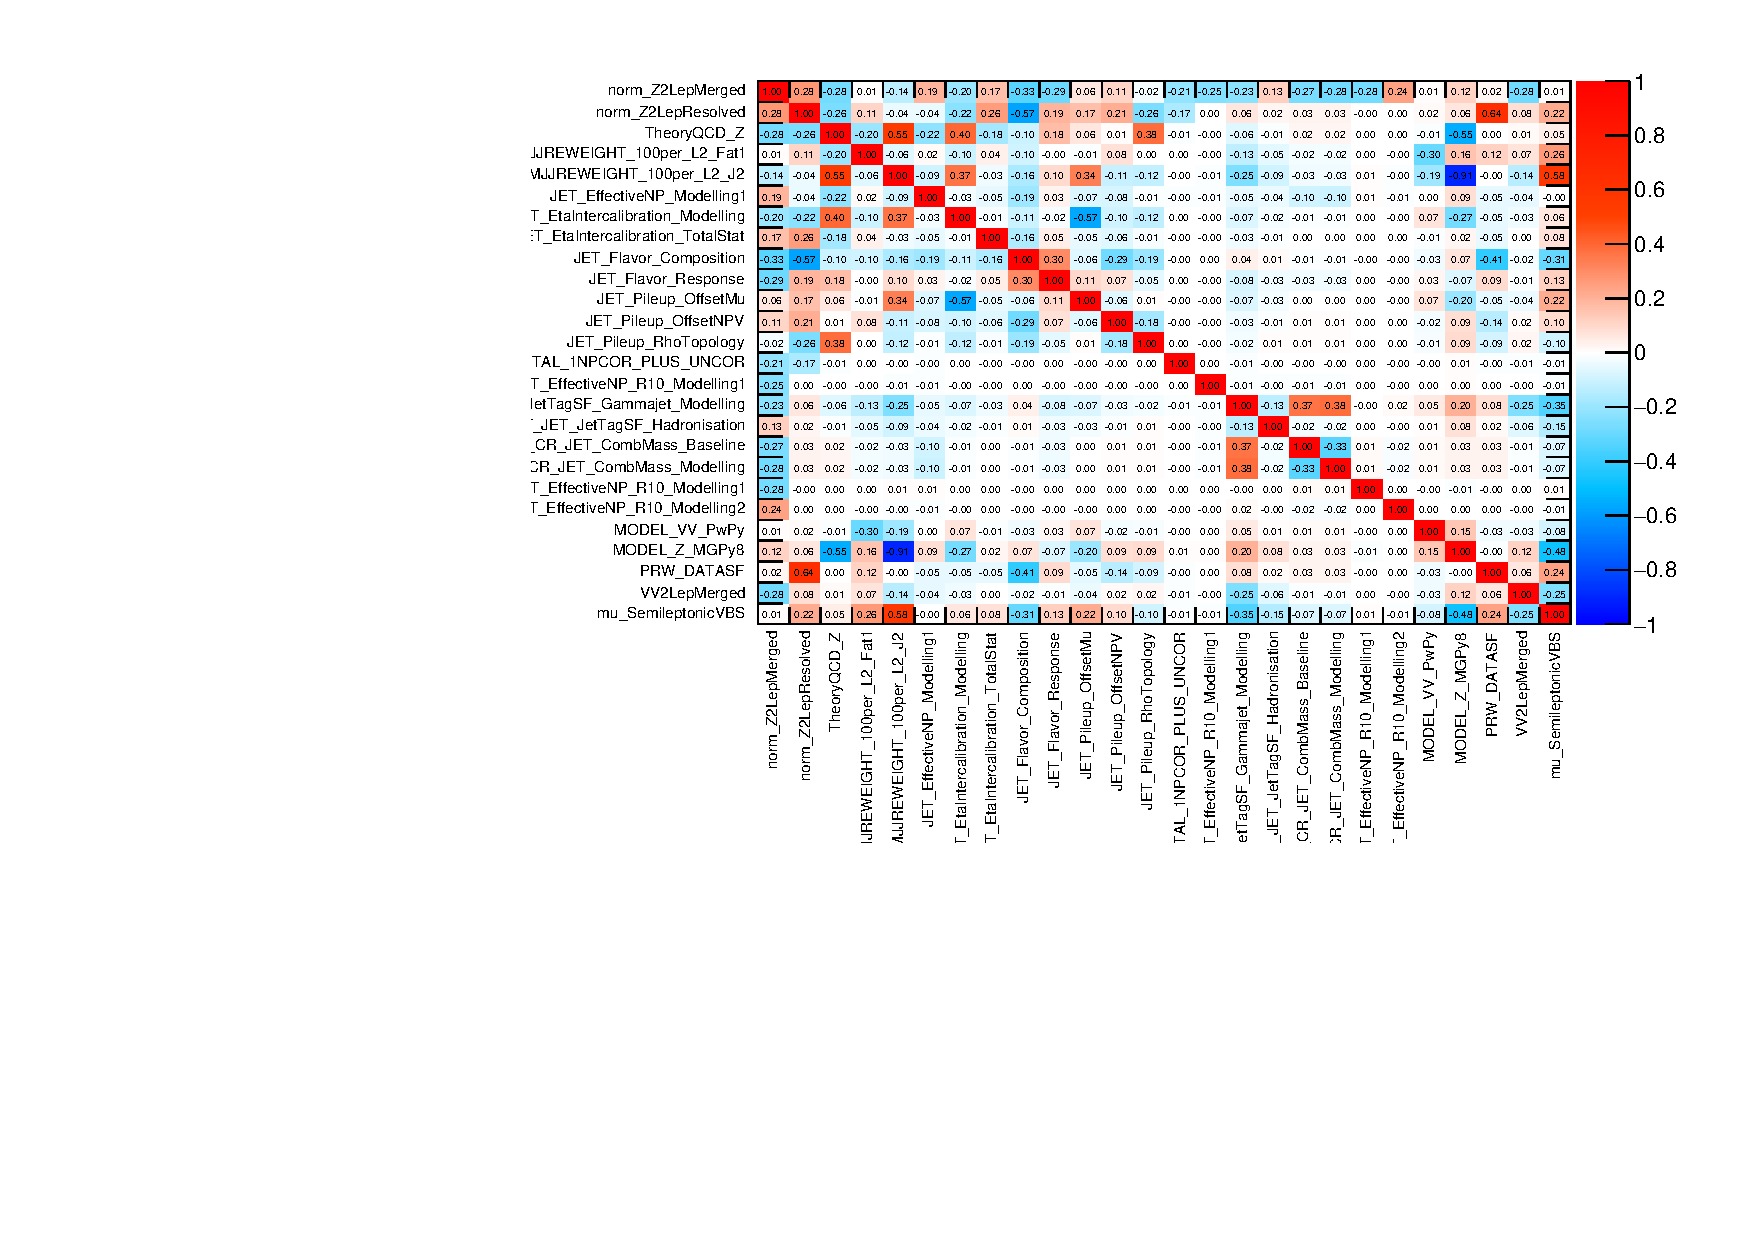
\includegraphics[width=\linewidth]{figures/2lep/FitResults/corr_HighCorrNoMCStat_DataLeftbins.pdf}
        \caption{Correlations for unconditional fit ($\mu=1$) to data in the left bins only, for the 2 lepton channel only.}
       \label{fig:fit_2lep_corr_left}
\end{figure}

Similar constraints as found in the Asimov fit are found and confirmed in the left bins only fit.
They have been already discussed.
In addition, some pulls are found, they are:

\begin{itemize}

       \item \texttt{SysTheoryQCD\_Z} it is coming from the data modelling of the left side bins;
       we will provide more checks in section \ref{sec:fit_decorrStudies}.

       \item \texttt{SysMODEL\_Z\_MGPy8} it is coming from the differences in the generators affecting our phase space;
       we can rely on the data fit for this uncertainty.

       \item \texttt{SysJET\_Pileup\_OffsetMu} is pile-up related uncertainty.
       This systematic uncertainty is expected to have a large shape effect on the forward jets.

       \item \texttt{SysFATJET\_FatJetTagSF\_Gammajet\_Modelling} this is the uncertainty related to the boosted tagger SF efficiency.
       We can see this pull since this uncertainty has a large effect in Merged CR.
\end{itemize}

%\section{Fitted Event Yields}
%\section{Prefit plots}
%\section{Postfit plots}
%\section{Nuisance Parameter Pulls}
%\section{Nuisance Parameter Correlations}
%\section{Ranking Plots}




